\documentclass[11pt, oneside]{book}

% Essential packages
\usepackage[T1]{fontenc}
\usepackage[utf8]{inputenc}
\usepackage[english]{babel}

% Mathematical packages and configuration
\usepackage{amsmath}
\usepackage{amssymb}
\usepackage{amsfonts}
\usepackage{amsthm}
\usepackage{mathtools}
\usepackage{siunitx}

% Aesthetic packages and configuration
\usepackage[colorlinks=true, linkcolor=blue]{hyperref}
\usepackage[margin=1.4in, footskip=0.2in]{geometry}
\usepackage[Sonny]{fncychap}

% Bibliography packages 
\usepackage{biblatex}
\usepackage{csquotes}
\addbibresource{references.bib}

% Other kind of packages
\usepackage{setspace}
\setstretch{1.05}
\usepackage{enumitem}
\usepackage{xargs}                      
\usepackage[pdftex,dvipsnames]{xcolor}  
\usepackage[colorinlistoftodos, prependcaption, textsize=footnotesize]{todonotes}
\usepackage{bm}

\usepackage{graphicx}
\usepackage{caption}
\usepackage{subcaption}

\newcommandx{\unsure}[2][1=]{\todo[linecolor=red, backgroundcolor=red!25,
bordercolor=red,#1]{#2}}
\newcommandx{\change}[2][1=]{\todo[linecolor=blue, backgroundcolor=blue!25,
bordercolor=blue,#1]{#2}}
\setlength{\marginparwidth}{3cm}

\theoremstyle{plain}
\newtheorem{thm}{Theorem}[section]
\newtheorem{lem}{Lemma}[thm]
\newtheorem{cor}{Corollary}[thm]
\newtheorem{prop}{Proposition}[section]
\newtheorem{defn}{Definition}[section]

\theoremstyle{remark}
\newtheorem*{rem}{Remark}

\DeclareMathOperator{\var}{var}
\DeclareMathOperator{\cov}{cov}
\newcommand*{\mbf}[1]{\mathbf{#1}}

\title{\textbf{Variations of Principal Component Analysis for Extremes and
Application to Climate Data}}
\author{Miguel Donderis de Vicente \hspace{3mm} NIU: 1491198}
\date{June 28, 2022}

\begin{document}
\maketitle

\tableofcontents
\thispagestyle{empty}

\mainmatter
\chapter{Introduction}
\chapter{Methods}

\section{Principal Component Analysis (PCA)}
Principal Component Analysis\change{no me termina de convencer esta
introducción} is probably the oldest and best known of all the existing
multivariate analysis techniques. It was first introduced in 1901 by Karl
Pearson, analogous to the Principal Axis Theorem in mechanics, and developed by
Harold Hotelling three decades later. Like almost all multivariate analysis
methods, it was not widely used until the advent of the first electronic
computers; but today it is widely available and is part of any statistical
package.

The central idea of Principal Component Analysis is to reduce the dimensionality
of a data set in which there are a large number of interrelated variables, while
preserving as much variability as possible. This reduction is achieved by
transforming this data into a new set of variables, called \emph{Main
Components}, which are uncorrelated with each other and which are ordered so
that the first components retain most of the dispersion present in the total set
of original data. The calculation of the main components is reduced to solving
an algebraic problem of calculating eigenvalues and eigenvectors for a positive
and symmetric semi-definite matrix. 

So as to do the analysis we will focus on the \cite{joliffe} paper.

\subsection{Definition and derivation of the Principal
Components}\label{sec:def-algderivation}
Let's suppose that $\mathbf{x} = (x_1,\dots,x_p)^\top\in\mathbb{R}^p$
is\change{this introduction does neither convince me at all. I should revise it
for sure} a vector of $p$ random variables such that the variances of these $p$
random variables and the structure of the covariances or correlations between
them are of interest. Unless $p$ is very small, or the structure of the
variables is very simple, it will often not be very helpful to look directly at
the $p$ variances and the $\frac{1}{2}p(p-1)$ covariances or correlations.
Therefore, an alternative approach is necessary, and the most optimal way is to
look for a few variables that preserve most of the information given by these
variances and covariances or correlations, what ara called the Principal
Components. Although the analysis for finding these components called
\emph{Principal Component Analysis}, which we will refer to as PCA from now on,
does not ignore covariances and correlations, it mainly concentrates on
variances.

The first step for finding the Principal Components is to look for a linear
combination $\bm{\alpha}_1^\top\mathbf{x}$ of the elements of $\mathbf{x}$ having
maximum variance, where $\bm{\alpha}_1\in\mathbb{R}^p$ is a vector such that
$\bm{\alpha}_1^\top\mathbf{x} = \alpha_{11}x_1 + \alpha_{12}x_2 + \cdots +
\alpha_{1p}x_p = \sum_{j=1}^p\alpha_{1j}x_j.$ Next, look for a second linear
combination $\bm{\alpha}_2\mathbf{x}$, uncorrelated with
$\bm{\alpha}_1\mathbf{x}$, having maximum variance, and so on, so that at
the $k$th step it is found a linear combination $\bm{\alpha}_k\mathbf{x}$
having maximum variance subject to being uncorrelated with the $k-1$ previous
linear combinations, $\bm{\alpha}_1^\top\mathbf{x},
\bm{\alpha}_2^\top\mathbf{x}, \dots, \bm{\alpha}_{k-1}^\top\mathbf{x}.$ The
$k$th derived variable, $\bm{\alpha}_k\mathbf{x}$, is called the $k$th Principal
Component, as stated before. It is clear that up to $p$ PCs can be found, as
much as the dimension of the original random vector, but it is hoped that most
of the variation of $\mathbf{x}$ will be accounted for by $m$ PCs, where $m\ll
p$. Generally, if a set of $p$ variables has substantial correlations among
them, then the first few PCs will account for most of the variation in the
original variables.  Conversely, the last few PCs identify directions of little
variation, that is, near-constant linear relationships among the original
variables. 

Having defined the PCs, we now need to understand how to find them. Consider,
for the moment, the case where the random vector $\mathbf{x}$ has known
covariance matrix $\mathbf{\Sigma}$, the matrix whose $(i,j)th$ element is the
covariance between the $i$th and the $j$th elements of $\mathbf{x}$ when $i\neq
j$ and the variance of the $i$th element when $i=j.$ The more realistic case in
which $\mathbf{\Sigma}$ is unknown follows by replacing it by a sample
covariance matrix $\mathbf{S}$. Then, it turns out that the $k$th PC is given by
$\mathbf{z}_k = \bm{\alpha}_k^\top\mathbf{x},\hspace{.25em} k=1,\dots,p,$ where
$\bm{\alpha}_k$ is an eigenvector of $\mathbf{\Sigma}$ corresponding to the
$k$th largest eigenvalue $\lambda_k$. Furthermore, if $\bm{\alpha}_k$ is chosen
to be normalized, then $\text{var}(\bm{z}_k) = \lambda_k$.  The following
algebraic derivation of the PCs is the standard one given in many multivariate
analysis books, and it may be skipped by those familiarized with this method.

Consider first the expression $\bm{\alpha}_1^\top\mathbf{x}$, where
$\bm{\alpha}_1$ is chosen to maximize $\text{var}(\bm{\alpha}_1^\top\mathbf{x})
= \bm{\alpha}_1^\top\mathbf{\Sigma}\bm{\alpha}_1$. We note that the maximum of
this expression will not be achieved for a finite $\bm{\alpha}_1$, so a
normalization constraint, $\bm{\alpha}_1^\top\bm{\alpha}_1 = 1$ must be imposed.
The standard approach to maximize the given expression subject to the
normalization constraint is to use the Lagrange multipliers technique. Hence,
maximize $\bm{\alpha}_1^\top\mathbf{\Sigma}\bm{\alpha}_1 -
\lambda(\bm{\alpha}_1^\top\bm{\alpha}_1 - 1)$, where $\lambda$ is the Lagrange
multiplier. Differentiation with respect to $\bm{\alpha}_1$ gives
$$\mathbf{\Sigma}\bm{\alpha}_1 - \lambda\bm{\alpha}_1 = (\mathbf{\Sigma} -
\lambda\mathbb{I}_p)\bm{\alpha}_1 = 0,$$ where
$\mathbb{I}_p\in\mathbb{R}^{p\times p}$ is the identity matrix. Thus, we note
that $\lambda$ is an eigenvalue of $\mathbf{\Sigma}$ and $\bm{\alpha}_1$ is its
corresponding eigenvector. So as to decide to which of the eigenvectors of
$\mathbf{\Sigma}$ does correspond, we recall that the quantinty to be maximized
is $$\text{var}(\bm{\alpha}_1^\top\mathbf{x}) =
\bm{\alpha}_1^\top\mathbf{\Sigma}\bm{\alpha}_1 =
\bm{\alpha}_1^\top\lambda\bm{\alpha}_1 = \lambda\bm{\alpha}_1^\top\bm{\alpha}_1
= \lambda,$$ so $\lambda$ must be as large as possible and therefore
$\mathbf{\alpha}_1$ is the eigenvector corresponding to the largest eigenvalue of
$\mathbf{\Sigma}$ and $\text{var}(\bm{\alpha}_1^\top\mathbf{x}) = \lambda_1$ the
largest eigenvalue. 

In general, the $k$th PC of $\mathbf{x}$ is $\bm{\alpha}_k^\top\mathbf{x}$ and
$\text{var}(\bm{\alpha}_k^\top\mathbf{x}) = \lambda_k$, where $\lambda_k$ is the
$k$th largest eigenvalue of $\mathbf{\Sigma}$ and $\bm{\alpha}_k$ is its
corresponding eigenvector. We now will derive this expression for the case
$k=2$, and the proof for $k\geq 3$  is slightly more complicated but similar in
the procedure. 

The second PC, $\bm{\alpha}_2^\top\mathbf{x}$, maximizes
$\text{var}(\bm{\alpha}_2^\top\mathbf{x}) =
\bm{\alpha}_2^\top\mathbf{\Sigma}\bm{\alpha}_2$ subject to being uncorrelated
with the first PC, $\bm{\alpha}_1^\top\mathbf{x}$, or equivalently subject to
the restriction $\text{cov}(\bm{\alpha}_1^\top\mathbf{x},
\bm{\alpha}_2^\top\mathbf{x}) = 0,$ where $\text{cov}(x,y)$ denotes the
covariance between $x,y$. Now,
$$\text{cov}(\bm{\alpha}_1^\top\mathbf{x},\bm{\alpha}_2^\top\mathbf{x}) =
\bm{\alpha}_1^\top\mathbf{\Sigma}\bm{\alpha}_2 =
\bm{\alpha}_2^\top\mathbf{\Sigma}\bm{\alpha}_1 =
\bm{\alpha}_2^\top\lambda\bm{\alpha}_1 =\lambda_1\bm{\alpha}_2^\top\bm{\alpha}_1
= \lambda_1\bm{\alpha}_1^\top\bm{\alpha}_2 = 0,$$ and any of the equations of
this equality can be used to specify uncorrelation between the two first PCs.
As again, we want to maximize $\text{var}(\bm{\alpha}_2^\top\mathbf{x})$ subject
to the normalization constraint, to make sure the variance is bounded, and to
the uncorrelation constraint, so the quantity to be maximized is now
$\bm{\alpha}_2^\top\mathbf{x}$ we have to maximize
$\bm{\alpha}_2^\top\mathbf{\Sigma}\bm{\alpha}_2 -
\lambda(\bm{\alpha}_2^\top\bm{\alpha}_2 - 1) -
\phi\bm{\alpha}_2^\top\bm{\alpha}_1,$ where $\lambda,\phi$ are the Lagrange
multipliers. Differentiating with respect to $\bm{\alpha}_2$ and multiplying by
$\bm{\alpha}_1^\top$ on the left we obtain
$$\bm{\alpha}_1^\top\mathbf{\Sigma}\bm{\alpha}_2 -
\lambda\bm{\alpha}_1^\top\bm{\alpha}_2 - \phi\bm{\alpha}_1^\top\bm{\alpha}_1 =
0,$$ and, since the first two terms are zero because of the uncorrelation
resctriction and $\bm{\alpha}_1^\top\bm{\alpha}_1 = 1,$ we obtain that $\phi=0$.
Therefore, the equation simplified is $\mathbf{\Sigma}\bm{\alpha}_2 -
\lambda\bm{\alpha}_2 = (\mathbf{\Sigma} - \lambda\mathbb{I})\bm{\alpha}_2 = 0,$
so $\lambda$ is once more an eigenvalue of $\bm{\Sigma}$ and $\bm{\alpha}_2$ is
its corresponding eigenvector. Again, the quantity to maximize is $\lambda =
\bm{\alpha}_2^\top\mathbf{\Sigma}\bm{\alpha}_2$. Assuming that $\mathbf{\Sigma}$
does not have repeated eigenvalues, as if it dit it would follow that
$\bm{\alpha}_2 = \bm{\alpha}_1$ violating the constraint of uncorrelation, we
have that $\lambda$ is the second largest eigenvalue of $\mathbf{\Sigma}$ and
$\bm{\alpha}_2$ is its corresponding eigenvector. As stated before, it can be
shown that for the third, fourth and so on PCs, the vectors of coefficients
$\bm{\alpha}_3, \bm{\alpha}_4,\dots, \bm{\alpha}_p$ are the eigenvectors of
$\mathbf{\Sigma}$ corresponding to $\lambda_3, \lambda_4,\dots,\lambda_p$, the
third, fourth until the smallest eigenvalue of $\mathbf{\Sigma}$, and
furthermore $\text{var}(\bm{\alpha}_k^\top\mathbf{x}) =
\lambda_k,\hspace{.25em}k=1,\dots,p.$ 

It should be noted that sometimes the eigenvectors $\bm{\alpha}_k$ are referred
to as Principal Components. This usage, though sometimes defended, is confusing
and it is preferable to reserve the term \emph{Principal Components} for the
derived variables $\bm{\alpha}_k^\top\mathbf{x}$, the projection of the data
vector $\mathbf{x}$ onto the $k$th eigenvector $\bm{\alpha}_k$,  which are also
called Empirical Orthogonal Variables, and denote by \emph{Empirical Orthogonal
Functions}, or EOFs, the vectors $\bm{\alpha}_k$, which are also called vector
of coefficients or loadings. Further discussion is provided in Appendix
\ref{chap:terminology-pca}.

\subsection{Optimal properties of Population Principal
    Components}\label{sec:optprop-pop}
Consider the derivation of the Principal Components given in the previous
section, and denote $\mathbf{z_k}$ the vector whose $k$th element is $z_k,$ the
$k$th Principal Component, $k=1,\dots,p.$. For ease of reading, henceforth we
will denote a Principal Component as PC.  Unless stated otherwise, the $k$th PC
will be taken to mean the component with the $k$th largest variance, with the
corresponding interpretations for the $k$th eigenvalue and the $k$th
eigenvector. Then, 
\begin{equation}\label{eq:pop-PC}
    \mathbf{z} = \mathbf{A'x},
\end{equation}
where $\mathbf{A'}$ is the orthogonal matrix whose $k$th column, $\alpha_k$, is
the $kth$ eigenvector of $\mathbf{\Sigma}.$ Hence, we note that the PCs are
defined by an orthonormal linear transformation of $\mathbf{x}$. Furthermore, we
have directly from the derivation in the previous section that 
\begin{equation}\label{eq:diag_sigma}
    \mathbf{\Sigma A}=\mathbf{A\Lambda},
\end{equation}
where $\mathbf{\Lambda}$ is the diagonal matrix whose
$k$th diagonal element is $\lambda_k$, the $k$th largest eigenvalue of
$\mathbf{\Sigma}$, such that $\lambda_k = \text{var}(\bm{\alpha'}_k\mathbf{x}) =
\text{var}(z_k).$ We observe two different ways of reexpressing this equality,
which follow because $\mathbf{A}$ is a orthogonal matrix and that will be useful
later, namely $\mathbf{A'\Sigma A} = \mathbf{\Lambda}$ and $\bm{\Sigma} =
\mathbf{A\Lambda A'}.$ The orthonormal linear transformation \eqref{eq:pop-PC}
of $\mathbf{x}$, which defines the PCs $\mathbf{z}$, has a number of optimal
properties which we will discuss.
\begin{prop}\label{prop:max_sigma}
    For any integer $q$, $1\leq q\leq p,$ consider the orthonormal linear
    transformation $$\mathbf{y} = \mathbf{B'x},$$ where
    $\mathbf{y}\in\mathbb{R}^q, \mathbf{B'}\in\mathbb{R}^{q\times p}$, and let
    $\mathbf{\Sigma}_y = \mathbf{B'\Sigma B}$ be the variance-covariance matrix
    for $\mathbf{y}$. Then the trace of $\mathbf{\Sigma}_y$, denoted
    $\emph{tr}(\mathbf{\Sigma}_y)$, is maximized by taking $\mathbf{B} =
    \mathbf{A}_q$, where $\mathbf{A}_q$ consists of the first $q$ columns of
    $\mathbf{A}$.  
\end{prop}    
\begin{proof}
    Let $\bm{\beta}_k$ be the $k$th column of $\mathbf{B}$. As the columns of
    $\mathbf{A}$ form a basis for a $p-$dimensional space, we have that
    $\bm{\beta}_k = \sum_{j=1}^p c_{jk}\bm{\alpha}_j,\hspace{.25em}
    k=1,\dots,q,$ where $c_{jk}, j= 1,\dots,p, k=1,\dots, q$ are appropiately
    defined constants. Hence, we have that $\mathbf{B} = \mathbf{AC},$ where
    $\mathbf{C}\in\mathbb{R}^{p\times q}$ with $(j,k)$th element $c_{jk}$, and
    we also observe that $$\mathbf{B'\Sigma B} = \mathbf{C'A'\Sigma AC} =
    \mathbf{C'\Sigma C} = \sum_{j=1}^p\lambda_j\mathbf{c}_j\mathbf{c}_j',$$
    where we denote $\mathbf{c}_j'$ the $j$th row of $\mathbf{C}$ and we have
    used equation \eqref{eq:diag_sigma} and the fact that $\mathbf{\Lambda}$ is a
    diagonal matrix. Therefore, $$\text{tr}(\mathbf{B'\Sigma B}) =
    \sum_{j=1}^p\lambda_j \text{tr}(\mathbf{c}_j\mathbf{c}_j') =
    \sum_{j=1}^p\lambda_j \text{tr}(\mathbf{c}_j'\mathbf{c}_j) =
    \sum_{j=1}^p\lambda_j\mathbf{c}_j'\mathbf{c}_j =
    \sum_{j=1}^p\sum_{k=1}^q\lambda_j c_{jk}^2.$$ Now, $\mathbf{C} =
    \mathbf{A'B},$ so $\mathbf{C'C} = \mathbf{B'AA'B} = \mathbf{B'B} =
    \mathbb{I}_q$, because $\mathbf{A}$ is orthogonal and the columns of
    $\mathbf{B}$ are orthonormal. Hence, $\sum_{j=1}^p\sum_{k=1}^qc_{jk}^2 = q,$
    and the columns of $\mathbf{C}$ are also orthonormal and it can be thought
    as the first $q$ columns of a orthogonal matrix
    $\mathbf{D}\in\mathbb{R}^{p\times p}.$ But note that the rows of
    $\mathbf{D}$ are orthonormal, i.e. $\mathbf{d}_j'\mathbf{d}_j =
    1,\hspace{.25em} j=1,\dots, p$. As the rows of $\mathbf{C}$ consist of the
    first $q$ elements of the rows of $\mathbf{D}$ it is clear that
    $\mathbf{c}_j'\mathbf{c}j\leq 1,\hspace{.25em}j=1,\dots,p$, and therefore
    $\sum_{k=1}^qc_{jk}^2\leq 1.$ Now, as we have seen $\sum_{k=1}^qc_{jk}^2\leq
    1$ is the coefficient of $\lambda_j,$ and the sum of these coefficients is
    $q$ and none of the coefficients can exceed 1. By construction of the PCs, 
    $\lambda_1>\lambda_2>\cdots\lambda_p,$ and we note that
    $\sum_{j=1}^p\left(\sum_{k=1}^qc_{jk}^2\right)\lambda_j$ will be maximized
    if we can find a set of coefficients $c_{jk}$ such that
    $$\sum_{k=1}^qc_{jk}^2 = 
    \begin{cases}
        1, & j=1,\dots,q,\\
        0, & j=q+1,\dots,p.
    \end{cases}$$ But if $\mathbf{B'} = \mathbf{A}_q',$ then
    $$c_{jk} =
    \begin{cases}
        1, & 1\leq j=k\leq q,\\
        0, & \text{elsewhere},
    \end{cases}$$ what satisfies the previous condition. Therefore,
    $\text{tr}(\mathbf{\Sigma}_y)$ is maximized by taking $\mathbf{B'} =
    \mathbf{A}_q',$ as required. 
\end{proof}    
\begin{prop}\label{prop:min_sigma}
    For any integer $q$, $1\leq q\leq p,$ consider the orthonormal linear
    transformation $$\mathbf{y} = \mathbf{B'x},$$ where
    $\mathbf{y}\in\mathbb{R}^q, \mathbf{B'}\in\mathbb{R}^{q\times p}$, and let
    $\mathbf{\Sigma}_y = \mathbf{B'\Sigma B}$ be the variance-covariance matrix
    for $\mathbf{y}$. Then $\emph{tr}(\mathbf{\Sigma}_y)$ is minimized by taking
    $\mathbf{B} = \mathbf{A}_q^*$, where $\mathbf{A}_q^*$ consists of the last 
    $q$ columns of $\mathbf{A}$
\end{prop}
\begin{proof}
    The derivation of the PCs given in the section \ref{sec:def-algderivation}
    can be easily turned around so as to succesively find linear functions of
    $\mathbf{x}$ whose variance is small as possible, subject to the constraint
    of being uncorrelated with the previous linear functions. One may note that
    the process is similar and that the only change is that, instead of
    maximizing the variance, it must be minimized. Therefore, the solutions are
    again the eigenvectors of $\mathbf{\Sigma}$, but this time in reverse order,
    starting with the one corresponding to the smallest variance. Thus, the
    proof for the Proposition \ref{prop:max_sigma} can be easily adapted to
    prove this case. 
\end{proof}
The statistical implications of Proposition \ref{prop:min_sigma} is that the
last few PCs are not just unstructured left-overs after removing the important
PCs, those which explain the greatest amount of variance. Because these last PCs
have variances as small as possible they are useful in their own right, for
example they can be used to detect unsuspected near-constant linear
relationships between the elements of $\mathbf{x}$, in selecting a subset of
$\mathbf{x}$ or in the detection of outliers. However, we will not focus on
these applications, but in the study of the components which explain the
greatest variance.
\begin{prop}[Spectral Decomposition of $\mathbf{\Sigma}$]\label{prop:specdecomp} 
    Let $\mathbf{x}$ be a vector with known covariance matrix $\mathbf{\Sigma}$.
    Then $$\mathbf{\Sigma} = \lambda_1\bm{\alpha}_1\bm{\alpha}_1' + 
    \lambda_2\bm{\alpha}_2\bm{\alpha}_2' + \cdots +
    \lambda_p\bm{\alpha}_p\bm{\alpha}_p'.$$
\end{prop}    
\begin{proof}
    From equation \eqref{eq:diag_sigma} we have that $\mathbf{\Sigma} =
    \mathbf{A\Lambda A'},$ and therefore expanding the right-hand side of the
    matrix product, as $\mathbf{\Lambda}$ is a diagonal matrix and $\mathbf{A}$
    is orthonormal, we get that $\mathbf{A\Lambda A'} = \sum_{k=1}
    \lambda_k\bm{\alpha}_k\bm{\alpha}_k'$, what shows that $\mathbf{\Sigma} =
    \sum_{k=1} \lambda_k\bm{\alpha}_k\bm{\alpha}_k',$ as required.
\end{proof}    
Looking at the diagonal elements we see that $\var(x_j) =
\sum_{k=1}^p\lambda_k\alpha^2_{kj}$. The implication of the present result is
that not only can we decompose the combined variances of all the elements of
$\mathbf{x}$ into decreasing contributions due to each PC, but we can also
decompose the whole covariance matrix into contributions
$\lambda_k\bm{\alpha}_k\bm{\alpha}_k^\top$ from each PC.
\begin{prop}\label{prop:max_det}
    For any integer $q$, $1\leq q\leq p,$ consider the orthonormal linear
    transformation $$\mathbf{y} = \mathbf{B'x},$$ where
    $\mathbf{y}\in\mathbb{R}^q, \mathbf{B'}\in\mathbb{R}^{q\times p}$, and let
    $\mathbf{\Sigma}_y = \mathbf{B'\Sigma B}$ be the variance-covariance matrix
    for $\mathbf{y}$. If $\emph{det}(\mathbf{\Sigma}_y)$ denotes the determinant
    of the covariance matrix of $\mathbf{y}$, then
    $\emph{det}(\mathbf{\Sigma}_y)$ is maximized when $\mathbf{B} =
    \mathbf{A}_q$.
\end{prop}    
\begin{proof}
    Consider an arbitrary integer $k$ such that $1\leq k\leq q$, and let $S_k$
    be the subspace of $p$-dimensional vectors orthogonal to
    $\bm{\alpha}_1,\dots,\bm{\alpha}_{k-1}$. Then, $\text{dim}(S_k) = p-k+1$,
    where $\text{dim}(S_k)$ denotes the dimension of the vector space $S_k$.
    Furthermore, the $k$th eigenvalue of $\mathbf{\Sigma}$, $\lambda_k$,
    satisfies $$\lambda_k = \sup\limits_{\bm{\alpha}\in S_k, \bm{\alpha\neq
    0}}\left\{\frac{\bm{\alpha'}\mathbf{\Sigma}\bm{\alpha}}{\bm{\alpha'\alpha}}
    \right\}.$$ Suppose that $\mu_1>\mu_2>\cdots\mu_q$ are the eigenvalues of
    $\mathbf{B'\Sigma B}$ and that
    $\bm{\gamma}_1,\bm{\gamma}_2,\dots,\bm{\gamma}_q$ are the corresponding
    eigenvectors. Let $T_k$ be the the subspace of $q$-dimensional vectors
    orthogonal to $\bm{\gamma}_{k+1},\dots,\bm{\gamma}_{q},$ with
    $\text{dim}(T_k) = k$. Then, for any non-zero vector $\bm{\gamma}$ in $T_k$
    it holds that $\bm{\gamma}'\mathbf{B'\Sigma
    B}\bm{\gamma}\geq \mu_k\lVert\bm{\gamma}\lVert.$ Consider now the
    subspace $\tilde{S}_k$ of $p$-dimensional vectors of the form
    $\mathbf{\Sigma}\bm{\gamma}, \bm{\gamma}\in T_k$. Then we have that
    $\text{dim}(\tilde{S}_k) = \text{dim}(T_k)=k$, because $\mathbf{B}$
    preserves lengths of vectors. From the Grassmann formula, we have that
    $$\text{dim}(S_k\cap\tilde{S}_k) + \text{dim}(S_k + \tilde{S}_k) =
    \text{dim}(S_k) + \text{dim}(\tilde{S}_k)$$. But as $\text{dim}(S_k +
    \tilde{S}_k)\leq p$, $\text{dim}(S_k) = p-k+1$ and $\text{dim}(\tilde{S}_k)
    = k$, necessarily $\text{dim}(S_k\cap\tilde{S}_k)\geq 1$. Therefore, there
    exists a non-zero vector $\bm{\alpha}\in S_k$ of the form $\bm{\alpha} =
    B\bm{\gamma}$ for a given $\bm{\gamma}\in T_k$, so it follows that $$\mu_k
    \leq \frac{\bm{\gamma}'\mathbf{B'\Sigma
    B}\bm{\gamma}}{\bm{\gamma}'\bm{\gamma}} = \frac{\bm{\gamma}'\mathbf{B'\Sigma
    B}\bm{\gamma}}{\bm{\gamma}'\mathbf{B'B}\bm{\gamma}} =
    \frac{\bm{\alpha'}\mathbf{\Sigma}\bm{\alpha}}{\bm{\alpha'\alpha}}\leq  
    \lambda_k.$$ Hence, the $k$th eigenvalue of $\mathbf{B'\Sigma B}$ is smaller
    than the $k$th eigenvalue of $\mathbf{\Sigma}$, $k=1,\dots,q.$ This means
    that $\text{det}(\mathbf{\Sigma}_y) = \prod_{k=1}^q\mu_k \leq
    \prod_{k=1}^q\lambda_k$, but if $\mathbf{B}=\mathbf{A}_q$ then
    $\text{det}(\mathbf{\Sigma}_y) = \prod_{k=1}^q\lambda_k$ in this case, and
    therefore $\text{det}(\mathbf{\Sigma}_y)$ is maximized when $\mathbf{B} =
    \mathbf{A}_q.$
\end{proof}    
The importance of this result follows because the determinant of the covariance
matrix, which is also called \emph{generalized variance} can be used as a single
measure of spread for a multivariate random vector. For multivariate normal
distributed random vector $\mathbf{x}$, the first $q$ PCs are $q$ linear
functions of $\mathbf{x}$ whose joint probability distribution has contours of
fixed probability enclosing the maximum volume. 
\begin{prop}\label{prop:minimumvar}
    Suppose that we wish to predict each random variable $x_j$ in $\mathbf{x}$
    by a linear function of $\mathbf{y}$, where
    $\mathbf{y}=\mathbf{B}'\mathbf{x}$. If $\sigma_j^2$ is the residual variance
    in predicting $x_j$ from $\mathbf{y}$, then $\sum_{j=1}^p\sigma_j^2$ is
    minimized if $\mathbf{B} = \mathbf{A}_q$.
\end{prop}    
The statistical implication of this result is that if we wished to get the best
linear predictor of $\mathbf{x}$ in a $q$-dimensional subspace, in the sense of
minimizing the sum over elements of $\mathbf{x}$ of the residual variances, then
this optimal $q$-dimensional subspace is defined by the first $q$
PCs.\unsure{population equivalent of proposition G3} Althoigh stated as an
algebraic property, it can be equally viewed geometrically. In fact, is the
population equivalent of Proposition CITE G3. It is interesting to note that the
PCs are the only set of $p$ linear functions of $\mathbf{x}$ that are
uncorrelated and have orthogonal vector of coefficients. A special case of
Proposition \ref{prop:minimumvar} was pointed out by Hotelling in
\cite{hotelling1933}, where ho noted that the first PCs derived from a
correlation matrix is the linear function of $\mathbf{x}$ that has greater mean
square correlation with the elements of $\mathbf{x}$ than any other function. 
\begin{prop}\label{prop:ellipsoids}
    Consider the family of $p$-dimensional ellipsoids
    $\mathbf{x}^\top\mathbf{\Sigma}^{-1}\mathbf{x} = \lambda$, where
    $\lambda\in\mathbb{N}$ is a constant. The PCs define the principal axes of
    these ellipsoids.
\end{prop}
\begin{proof}
    The PCs are defined by the transformation $\mathbf{z} =
    \mathbf{A}^\top\mathbf{x}$ and since $\mathbf{A}$ is a orthogonal matrix we
    can find the inverse transformation, given by $\mathbf{x} = \mathbf{Az}$.
    Then, substituing into the equation that describes a family of
    $p$-dimensional ellipsoids we find that
    $(\mathbf{Az})^\top\mathbf{\Sigma}^{-1}(\mathbf{Az}) = \mathbf{z}^\top
    \mathbf{A}^\top\mathbf{\Sigma}^{-1}\mathbf{Az}$. It is known that the
    eigenvectors of $\mathbf{\Sigma}^-1$ are the same as those of
    $\mathbf{\Sigma}$, and that the eigenvalues are the reciprocal, if we assume
    they are all strictly positive. From equation \eqref{eq:diag_sigma} that
    $\mathbf{A}\mathbf{\Sigma}^{-1}\mathbf{A} = \mathbf{\Lambda}^{-1}$, and
    therefore $\mathbf{z}^\top\mathbf{\Lambda}^{-1}\mathbf{z} =
    \sum_{k=1}^p\frac{z_k^2}{\lambda_k} = \lambda$, which is the equation of an
    ellipsoid referred to its principal axes. 
\end{proof}    
This result is important above all if the random vector $\mathbf{x}$ has a
multivariate normal distribution, as in this case the ellipsoids define contours
of constant probability. The interpretation of PCs as defining the principal
axes of ellipsoids of constant density was also mentioned by Hotelling in
\cite{hotelling1933}.\unsure{I'm not really sure wether to include this
proposition or not}
\begin{prop}\label{prop:max-expectationdistance}
    Suppose that $\mathbf{x}_1, \mathbf{x}_2$ are two independent random
    vectors, both having the same probability distribution and both subjected to
    the same linear transformation $\mathbf{y}_i = \mathbf{B}^\top\mathbf{x}_i$,
    $i=1,2$. If $\mathbf{B}\in\mathbb{R}^{p\times q}$ is a matrix with
    orthonormal columns chosen to maximize
    $\mathbb{E}[(\mathbf{y}_1-\mathbf{y}_2)^\top(\mathbf{y}_1\mathbf{y}_2)]$,
    then $\mathbf{B} = \mathbf{A}_q$.
\end{prop}    
\begin{proof}
    First, note that $\mathbf{x}_1$ and $\mathbf{x}_2$ have the same mean
    $\bm{\mu}$ and covariance matrix $\mathbf{\Sigma}$. Hence, $\mathbf{y}_1$
    and $\mathbf{y}_2$ also have the same mean and covariance matrix,
    $\mathbf{B}^\top\mathbf{\mu}$ and $\mathbf{B}^\top\mathbf{\Sigma}\mathbf{B}$
    respectively. Then,
    $$\mathbb{E}[(\mathbf{y}_1-\mathbf{y}_2)^\top(\mathbf{y}_1-\mathbf{y}_2)] =
    \mathbb{E}[(\mathbf{y}_1-
    \mathbf{B}^\top\bm{\mu})^\top(\mathbf{y}_1 - \mathbf{B}^\top\bm{\mu})] 
    \mathbb{E}[(\mathbf{y}_2-
    \mathbf{B}^\top\bm{\mu})^\top(\mathbf{y}_2 - \mathbf{B}^\top\bm{\mu})],  
    $$ where the cross-products vanish because of the independence of the random
    vectors. Now, for $i=1,2$ we have that 
    $\mathbb{E}[(\mathbf{y}_i-
    \mathbf{B}^\top\bm{\mu})^\top(\mathbf{y}_i - \mathbf{B}^\top\bm{\mu})]
    =\text{tr}(\mathbf{B}^\top\mathbf{\Sigma B},$ which is maximized when
    $\mathbf{B} = \mathbf{A}_q$ and as the present criterion has been shown to
    be $2\text{tr}(\mathbf{B}^\top\mathbf{\Sigma B}$ we have the desired result.
\end{proof}    
This property says that the expected Euclidean distance in a $q$-dimensional
subspace between two vectors of $p$ random variables with the same distribution
is made as large as possible if the subspace is defined by the first $q$ PCs.
Finally, this property can be of course reversed in the sense that
$\mathbb{E}[(\mathbf{y}_1-\mathbf{y}_2)^\top(\mathbf{y}_1\mathbf{y}_2)]$ is
minimized by taking $\mathbf{B} = \mathbf{A}_q^*$     

\subsection{Optimal properties of Sample Principal
    Components}\label{sec:optprop-sample}
In this section we will study some interesting and important algebraic and
geometric properties of PCs obtained from a sample covariance matrix, instead of
from a population covariance matrix. Most of these properties are just the
sample analogous of the population case, so they will be mentioned briefly, but
in addition there are other properties that are relevant only to sample PCs, so
these ones will be discussed more deeply.

Before deepening into the properties by themselves, we need to set some
notation. Suppose that we have $n$ different observations on the $p$-dimensional
random vector $\mbf{x}$, which we will denote by $\mbf{x}_1, \mbf{x}_2, \dots,
\mbf{x}_n$. Let $\tilde{z}_{i1} = \mbf{a}_1^\top\mbf{x}_i$, $i=1,\dots,n$ and
choose the vector of coefficients $\mbf{a}_1^\top$ to maximize the sample
variance $\frac{1}{n-1}\sum_{i=1}^n(\tilde{z}_{i1} - \bar{z}_1)^2$ subject to
the normalization constraint $\lVert\mbf{a}_1\lVert = 1$. Next, let
$\tilde{z}_{i2} = \mbf{a}_2^\top\mbf{x}_i$, $i=1,\dots,n$ and choose
$\mbf{a}_2^\top$ to maximize the sample variance of $\tilde{z}_{i2}$ subject to
the normalization constraint $\lVert\mbf{a}_2\lVert = 1$ and so that
$\tilde{z}_{i2}$ is uncorrelated with $\tilde{z}_{i1}$. One may note that this
process is similar to the one described in the section
\ref{sec:def-algderivation}, so continuing in an obvious manner we obtain a
sample version of the definition of PCs.  Therefore, $\tilde{\mbf{z}}_k =
\mbf{a}_k^\top\mbf{x} = (\tilde{z}_{ik},\dots, \tilde{z}_{in}$ is defined as the
$k$th sample PC, $k=1,\dots,p$, and $\tilde{z}_{ik}$ is the score of the $i$th
observation on the $k$th PC. If the derivation of section
\ref{sec:def-algderivation} is followed but with sample variances and
covariances replacing the population quantities, it turns out that the sample
variance of the PC scores for the $k$th sample is $l_k$, the $k$th largest
eigenvalue of the sample covariance $\mbf{S}$ of $\mbf{x} = (\mbf{x}_1,\dots,
\mbf{x}_n)$, and $\mbf{a}_k$ is the corresponding eigenvector for $k=1,\dots,p$. 

Define the matrices $\tilde{\mbf{X}}, \tilde{\mbf{Z}}\in\mathbb{R}^{n\times p}$
to have $(i,k)$th elements equal to the value of the $k$th element
$\tilde{x}_{ik}$ of $\mbf{x}_i$ and $\tilde{z}_{ik}$ of $\tilde{\mbf{z}}_i$.
Then, $\tilde{\mbf{X}}, \tilde{\mbf{Z}}$ are related by $\tilde{\mbf{Z}} =
\tilde{\mbf{X}}\mbf{A}$, where $\mbf{A}\in\mathbb{R}^{p\times p}$ is the
orthogonal matrix whose $k$th column is $\mbf{a}_k$. 

As the mean of $\mbf{x}$ is usually unkown, the $(j,k)th$ element of $\mbf{S}$
is
$\frac{1}{n-1}\sum_{i=1}^n(\tilde{x}_{ij}-\bar{x}_j)(\tilde{x}_{ik}-\bar{x}_k)$,
where $\bar{x}_j = \frac{1}{n}\sum_{i=1}^n\tilde{x}_{ij}$, $j=1,\dots,p$. The
matrix $\mbf{S}$ can be therefore written as $\mbf{S} =
\frac{1}{n-1}\mbf{S}^\top\mbf{S}$, where $\mbf{X}\in\mathbb{R}^{n\times p}$ is
the matrix whose $(i,j)th$ element is $(\tilde{x}_{ij}-\bar{x}_j)$, the $i$th
observation of the $j$th variable measured about its mean $\bar{x}_j$. Hence, a
convenient notation to define the PC scores is $\mbf{Z} = \mbf{XA}$, rather than
the earlier definition. Now, the PC scores will have exactly the same variances
and covariances as those given by $\tilde{\mbf{Z}}$ but will have zero mean.

Turning to the optimal algebraic properties listed in the section
\ref{sec:optprop-pop}, if we consider the orthonormal linear
transformation $\mbf{y}_i = \mbf{B}^\top\mbf{x}_i$, $i=1,\dots,n$, where
$\mbf{B}\in\mathbb{R}^{p\times q}$ is a orthonormal matrix, then Proposition
\ref{prop:max_sigma}, \ref{prop:min_sigma}, \ref{prop:max_det} and
\ref{prop:minimumvar} still hold, but replacing $\mbf{\Sigma}_y$ with the sample
covariance matrix of the observations $\mbf{y}_i$, $i=1,\dots,n,$ and with the
matrix $\mbf{A}$ defined as having as $k$th column the vector $\mbf{a}_k$ and
$\mbf{A}_q, \mbf{A}_q^*$ representing the first and last $q$ columns of
$\mbf{A}$, respectively. All proofs are similar to the ones given in section
\ref{sec:optprop-pop} by replacing the population quantities with the
corresponding sample quantities. Regarding Proposition \ref{prop:minimumvar}, to
which we didn't give a proof, it will reappear later as an important result an
will be proved.  Regarding the spectral decomposition, Proposition
\ref{prop:specdecomp} also hold for the sample case in the form $$\mbf{S} =
l_1\mbf{a}_1\mbf{a}_1^\top + l_2\mbf{a}_2\mbf{a}_2^\top + \cdots
l_p\mbf{a}_p\mbf{a}_p^\top.$$ The statistical implications of these properties
are esentially the same as the ones stated, but they must now be viewed in a
sample context.
\begin{prop} 
Suppose that $\mbf{X}$ consists of $n$ observations on $p$ predictor variables
$\mbf{x}$ measured about their sample means, and that the corresponding
regression equation is $\mbf{y} = \mbf{X}\bm{\beta} + \bm{\varepsilon}$, where
$\mbf{y}$ is the vector of $n$ observations of the dependent variable, again
measured about the sample mean. Suppose that $\mbf{X}$ is transformed by the
equation $\mbf{Z} = \mbf{XB}$, where $\mbf{B}\in\mathbb{R}^{p\times p}$ is a
orthogonal matrix. The regression equation can then be rewritten as $\mbf{y} =
\mbf{Z}\bm{\gamma} + \bm{\varepsilon},$ where $\bm{\gamma} =
\mbf{B}^{-1}\bm{\beta}$. The usual least square estimator for $\bm{\gamma}$ is
$\hat{\bm{\gamma}} = (\mbf{Z}^\top\mbf{Z})^{-1}\mbf{Z}^\top\mbf{y}$. Then the
elements of $\hat{\bm{\gamma}}$ have successively the smallest possible
variances if $\mbf{B} = \mbf{A}$, the matrix whose $k$th column is the $k$th
eigenvector of $\mbf{S}$. Hence, $\mbf{Z}$ consists of values of the sample
Principal Components for $\mbf{x}$.\unsure{unsure to include this proposition
and its proof} 
\end{prop}
\begin{proof}
    The proof is a bit weird and this proposition is also a  bit disconnected
    from the general overview of PCA, so by the moment I will not include it. 
\end{proof}    
This proposition implies that replacing the predictor variables in a regression
analysis by their first few PCs is a good idea

However, most of the optimal properties of PCs specific to sample situation are
geometric, or at least have an important geometric point of view. We now
introduce and discuss some of the most relevant ones. As with the algebraic
properties, the two geometric properties that we introduced in the population
case are still relevant for the sample PCs, although with slight modifications
to the statistical implications. Proposition \ref{prop:ellipsoids} is still
valid for samples but by replacing $\mbf{\Sigma}$ by $\mathbf{S}$. The
ellipsoids $\mbf{x}^\top\mbf{S}^{-1}\mbf{x} = \lambda$, where $\lambda$ is a
given constant, do not longer have the interpretation of countours of fixed
probability. In this case, these ellipsoids give contours of equal Mahalanobis
distance from the sample mean $\bar{\mbf{x}}$. That is why some authors have
interpreted PCA as successively finding orthogonal directions for which the
Mahalanobis distance from the set to a hypersphere enclosing all the data is
minimized. 

Regarding Proposition \ref{prop:max-expectationdistance}, it may also
be carried over from populations to samples. Suppose that the observations
$\mbf{x}_1,\mbf{x}_2,\dots,\mbf{x}_n$ are transformed by the orthonormal linear
transformation $\mbf{y}_i = \mbf{B}^\top\mbf{x}_i$, $i=1,2,\dots,n,$ where
$\mbf{B}\in\mathbb{R}^{p\times q}$ is a orthonormal matrix, so that
$\mbf{y}_1,\mbf{y}_2,\dots,\mbf{y}_n$ are projections of
$\mbf{x}_1,\mbf{x}_2,\dots,\mbf{x}_n$ onto a $q$-dimensional subspace. Then,
$$\sum_{h=1}^n\sum_{i=1}^n(\mbf{y}_h-\mbf{y}_i)^\top(\mbf{y}_h-\mbf{y}_i)$$ is
maximized when $\mbf{B} = \mbf{A}_q$. Conversely, the same quantity is minimized
when $\mbf{B} = \mbf{A}_q^*.$ This property, which for the population case
seemed irrelevant or at least out of context, for the sample case is very
important. This property means that if the $n$ observations are projected onto a
$q$-dimensional subspace, then the sum of squared Euclidean distances between
all pair of observations in the subspace is maximized when the subspace is
defined by the first $q$ PCs, the PCs that account for the greatest part of the
variance, while it is minimized when the subspace is defined by the last $q$
PCs. The proof that this property holds is similar to the population case, so we
will not repeat it. 

The next property is the sample equivalent to Proposition \ref{prop:minimumvar},
and both are concerned with least squares linear regression of each variable
$x_j$ on the $q$ variables contained in $\mbf{y}$.
\begin{prop}\label{prop:min-squaredistance}
    Suppose that the observations $\mbf{x}_1l, \mbf{x}_2, \dots, \mbf{x}_n$ are
    transformed by the orthonormal linear transformation $\mbf{y}_i =
    \mbf{B}^\top\mbf{x}_i$, $i=1,\dots,n,$ where $\mbf{B}\in\mathbb{R}^{p\times
    q}$ is a orthonormal matrix, so that $\mbf{y}_1, \mbf{y}_2, \dots,
    \mbf{y}_n$ are projections of $\mbf{x}_1, \mbf{x}_2, \dots, \mbf{x}_n$ onto
    a $q$-dimensional subspace. A measure of ``goodness of fit" of this
    $q$-dimensional subspace to $\mbf{x}_1, \mbf{x}_2, \dots, \mbf{x}_n$ can be
    defined as the sum of squared perpendicular distances of $\mbf{x}_1,
    \mbf{x}_2, \dots, \mbf{x}_n$ from the subspace. This measure is minimized
    when $\mbf{B} = \mbf{A}_q$.
\end{prop}    
\begin{proof}
\end{proof}    

\section{Extreme Principal Component Analysis (xPCA)}
\subsection{Regular variation. Definition and first properties}
The theory of regularly varying functions is an essential analytical tool for
dealing with heavy tails, long-range dependence and domains of attraction.
Roughly speaking, \emph{regularly varying functions} are those functions which
behave asymptotically like power functions, i.e. functions that are jointly
heavy tailed. In this section we will consider only real functions of a real
single variable and in the following sections we will considerate the
multivariate case for which we will have to introduce concepts such as vague
convergence. 

\begin{defn}
    A measurable function $U:\mathbb{R}^+\to\mathbb{R}^+$ is regularly varying
    at $\infty$ with index $\rho\in\mathbb{R}$, denoted by $U\in\text{RV}_\rho$,
    if for $x>0$, $$\lim_{t\to\infty}\frac{U(tx)}{U(t)} = x^\rho.$$ The exponent
    $\rho$ is called the exponent of variation.
\end{defn}    

\subsection*{A maximal domain of attraction}
Suppose that $\{X_n, n\geq 1\}$ are independent identically distributed random
variables with common distribution $F(x)$. The extreme is defined by the
following expression $M_n = \bigvee_{i=1}^n X_i = \text{max}\{X_1,\dots,X_n\}.$


\subsection*{Vague convergence}

\subsection{Extension of regular variation}
Resnick \cite{resnick2007} provides a comprehensive treatment of multivariate
regular variation. Roughly speaking, a random vector is said to be
\emph{multivariate regular-varying} if its joint tail decays like a power
function, in other words, it is jointly heavy-tailed. Although regular variation
can be defined on $\mathbb{R}^p$, during all this work we will consider it in
the nonnegativa orthant, as done in \cite{cooley-thibaud}, as this allows to
focus our attention on the direction for which we want to assess risk. 
\begin{defn}
    A random vector $\mathbf{X}$ that takes values in $\mathbb{R}^p_+ =
    [0,\infty)^p$ is said to be regularly varying if there exists a sequence
    $b_n\to\infty$ and a limit measure $\nu_\mathbf{X}$ for sets in
    $[0,\infty)^p\backslash\{0\}$ such that
    $n\mathbb{P}(b_n^{-1}\mathbf{X}\in\cdot)\xrightarrow{v}\nu_\mathbb{X}(\cdot)$
    as $n\to\infty$, where $\xrightarrow{v}$ denotes vague convergence in
    $M_+([0,\infty)),$ the space of nonnegative Radon measures on
    $[0,\infty)^p\backslash\{0\}$.
\end{defn}    
It can be shown that $b_n=L(n)n^{\frac{1}{\alpha}},$ where $L(\cdot)$ is some
slowly varying function and $\alpha>0$ is called the \emph{tail index} of
$\mathbf{X}$. We then write $\mathbf{X}\in\text{RV}^p_+(\alpha)$ so as to denote
a regularly varying random vector $\mathbf{X}$ with tail index $\alpha$.
Furthermore, the measure $\nu_\mathbf{X}$ has the scaling property, namely
$\nu_\mathbf{X}(aC) = a^{-\alpha}\nu_\mathbf{X}(C),$ for any set
$C\subset[0,\infty)^p\backslash\{0\}$ and any $a>0$. 

The scaling property implies that $\nu_\mathbf{X}$ can be more easely understood
for sets defined by polar, rather than cartesian, coodinates. Hence, given any
norm $\lVert\cdot\lVert$, the unit sphere is defines as $\mathbb{S}_{p-1}^+=
\{x\in \mathbb{R}^p_+: \lVert x\lVert=1\}.$ Now, we define the set $C(r,B) =
\{x\in\mathbb{R}^p_+: \lVert x\lVert >r, \frac{x}{\lVert x\lVert}\in B\},$ for
$r>0$ and $B\subset \mathbb{S}_{p-1}^+$ a Borel set. Then,
$\nu_\mathbf{X}\{C(r,B)\} = r^{-\alpha}H_\mathbf{X}(B)$, where $H_\mathbf{X}$ is
termed the angular measure on $\mathbf{S}^+_{p-1}$.

Consequently, $\nu_\mathbf{X}\{C(r,B)\} = r^{-\alpha}H_\mathbf{X}(B).$ The scale
of $\mathbf{X}$ is related to $\{b_n\}$ and $\nu_\mathbf{X}$ or $H_\mathbf{X}$.
If we now replace the sequence $\{b_n\}$ for $\{kb_n\},$ for some $k>0$, then
for any $r>0$ and $B\subset\mathbb{S}_{p-1}^+$ such that $C(r,B)$ is a
continuity set of $\nu_X$, then $n\mathbb{P}\{(kb_n)^{-1}\mathbf{X}\in C(r,B)\}
\to \nu_\mathbf{X}^\text{alt}\{C(r,B)\} = r^{-\alpha}H_\mathbf{X}^\text{alt}(B)$
, where $\nu_\mathbf{X}^\text{alt} = k^{-\alpha}\nu_\mathbf{X}$ and
$H_\mathbf{X}^\text{alt} = k^{-\alpha}H_\mathbf{X}$. We ackowledge this
relationship between $\{b_n\}, \nu_\mathbf{X}$ and $H_\mathbf{X}$ by saying that
$\mathbf{X}$ has limiting measure $\nu_\mathbf{X}$ and limiting angular measure
$H_\mathbf{X}$ when normalized by the succession $\{b_n\}$.

\subsection{Inner product space via transformation}
In the following section we describe the framework for defining an inner product
space on a given open set. We then use this framework so as to define a
particular inner product space on its positive orthant, whose operations
preserve regular variation. 

Let $t$ be a bijection from $\mathbb{R}$ onto some open set $\mathbb{X}\subset
\mathbb{R}$, and let $t^{-1}$ be its inverse. We will refer to $t$ as the
\emph{transform}. Let $\mathbb{X}^p$ be the set of $p-$dimensional vectors whose
elements lie on $\mathbb{X}$, i.e. if $\mathbf{x} = (x_1,\dots,x_p)
\in\mathbb{X}^p,$ then $x_i\in\mathbb{X},\hspace{0.25em}\forall x=1,\dots,p$. We
denote by $t(y)$ the elementwise application of the transform $t$ to the
elements of a given vector $y\in\mathbb{R}^p$, in such a way that other
functions operating on vectors will similarly be applied elementwise. We define
the vector addition of two elements $x_1,x_2\in\mathbb{X}^p$ by $x_1\oplus x_2 =
t\left(t^{-1}(x_1) + t^{-1}(x_2)\right).$ Given a real number $a\in\mathbb{R}$,
we define the scalar multiplication by a vector $x\in\mathbb{X}^p$ by $a\circ x
= t\left(at^{-1}(x)\right).$ We finally define the additive identity in
$\mathbb{X}^p$ as $0_{\mathbb{X}^p} = t(0)$ and the additive inverse of any
$x\in\mathbb{X}^p$ by $-x = t\left(-t^{-1}(x)\right)$. In the appendix section
\label{sec:vec-space} we show that the space $\mathbb{X}^p$ is in fact a vector
space.

Following the construction of the vector space $\mathbb{X}^p,$ let
$x_j\in\mathbb{X}^p$ and $a_j\in\mathbb{R},\hspace{.25em} j=1,\dots,q$, we
define a linear combination as $$a_1\circ x_1\oplus a_2\circ
x_2\oplus\cdots\oplus a_q\circ x_q = t\left(\sum_{j=1}^qa_jt^{-1}(x_j)\right).$$
We note that, as $\mathbb{X}^p$ is a $p-$dimensional vector space, any set of
$p$ vectors that are linearly independent in $\mathbb{X}^p$, namely vectors such
that if $a_1\circ x_1\oplus\cdots\oplus a_qx_q = 0$ then $a_j=0,\hspace{.25em}
j=1,\dots,q,$ will form a basis for $\mathbb{X}^p.$ 

Let now be $A=(\tilde{a}_1,\dots,\tilde{a}_q)\in\mathbb{R}^{p\times q}$ a matrix
of real numbers. Then, for a vector $x\in\mathbb{X}^q$ we define the matrix
multiplication by $A$ as $A\circ x = a_1\circ x_1\oplus\cdots\oplus a_q\circ
x_q = t\left(At^{-1}(x)\right)\in\mathbb{X}^p.$ If we denote
$\mathbb{I}\in\mathbb{R}^p$ the identity matrix, then $\mathbb{I}\circ x =
t\left(It^{-1}(x)\right) = x,$ and we note that if $B\in\mathbb{R}^{p'\times
p},$ then $B\circ A\circ x = B\circ t\left(At^{-1}(x)\right) =
t\left(BAt^{-1}(x)\right) = BA\circ x\in\mathbb{X}^{p'}.$ Now that we've
defined matrix multiplication in our particular vector space, we recall that as
in $\mathbb{R}^p,$ linear combinations can be written as matrix operations.
However, because of the fact that constants $a_j\in\mathbb{R}$ and vectors
$x_j\in\mathbb{X}^p\hspace{.25em}\forall j=1,\dots,n$, the linear combination in
this case can be reexpressed as $$a_1\circ x_1\oplus\cdots\oplus a_q\circ x_q =
Y\circ t(a),$$ where $Y\in\mathbb{R}^{p\times q}$ is the matrix whose columns
are $y_j=t^{-1}(x_i),\hspace{.25em}j=1,\dots,q.$

Given two vectors $x_1,x_2\in\mathbb{X}^p$, we define the scalar product in
$\mathbb{X}^p$ by $\langle x_1,x_2\rangle =
\sum_{i=1}^pt^{-1}(x_{1i})t^{-1}(x_{2i}).$ In the Appendix section ? we prove
that the conditions for being a well defined scalar product are met. We define
the norm of a vector $x\in\mathbb{X}^p$ as $\lVert x\lVert = \langle
x,x\rangle^\frac{1}{2}$ and say that two vectors $x_1,x_2\in\mathbb{X}^p$ are
orthogonal if $\langle x_1,x_2\rangle=0$, denoted by $x_1\perp x_2$. Now,
vectors $x_1,x_2\in\mathbb{X}^p$ and their preimages, $y_1=t^{-1}(x_1),
y_2=t^{-1}(x_2)\in\mathbb{R}^p$ share the same inner product value.
Consequently, $\lVert x\lVert = \lVert y\lVert_2$, and $x_1\perp x_2$ if and
only if $y_1\perp y_2\in\mathbb{R}^p.$

Let's consider now a nonsigular matrix $S\in\mathbb{R}^{p\times p}$ and think
of the linear transformation associated with it, $S:\mathbb{R}^p\to\mathbb{R}^p,$
defined by $x\mapsto S\circ x.$ We therefore define the inverse operator, and
$S^{-1}$ its associated matrix, to be an application such that
$S^{-1}\circ(S\circ x) = S\circ(S^{-1}\circ x) = x.$ We note that the inverse
operator coincides with the usual multiplication by the inverse matrix. 

If $S$ is a diagonalizable matrix, we can define the eigenvalue/eigenvector pair
of $S$ to be $\lambda\in\mathbb{R}$ and $e\in\mathbb{X}^p$ such that $S\circ e =
\lambda\circ e,$ where we assume that $\lVert e\lVert = 1$. Now, if $\lambda,$
$u$ are its corresponding eigenvalue/eigenvector pair in $\mathbb{R}^p$, then it
holds that $\lambda$ and $e=t(u)$ form an eigenvalue/eigenvector pair in
$\mathbb{X}^p$, i.e. $S\circ e = t(Su) = t(\lambda u) = \lambda\circ e.$
Further, we assume that $S$ is a symmetric positive definite matrix, namely
$y^TSy>0$ for any $y\in\mathbb{R}^p\backslash\{0\}$. We therefore define a
positive quadratic form im $\mathbb{X}^p$, whose associated matrix is $S$, by
$Q(S,x) = \langle x, S\circ x\rangle.$ In fact, we observe that $$Q(S,x) =
\langle x,t\left(St^{-1}(x)\right)\rangle = \sum_{i=1}^p\sum_{j=1}^p
t^{-1}(x_i)s_{ij}t^{-1}(x_j) = y^TSy,$$ where $y = t^{-1}(x).$ Hence, we see
that $x$ and its inverse image share the same quadratic form with respect to a
symmetric positive-definite matrix $S$. Consequently, relationships between the
eigenvectors and eigenvalues of $S$ and bounds on the quadratic forms in
$\mathbb{R}^p$ carry over to $\mathbb{X}^p$, yielding the following proposition
whose proof follows from linear algebra results in $\mathbb{R}^p$ in
\cite{johnson-wichern}.
\begin{prop}
    Let $S\in\mathbb{R}^{p\times p}$ be a diagonalizable matrix with real
    coefficients and $\lambda_1\geq\lambda_2\geq\dots\geq\lambda_p> 0$ and
    $u_1,u_2,\dots,u_p$ be the ordered eigenvalue/eigenvector pairs of the given
    matrix, and let $e_i = t(u_i),\hspace{.25em}i=1,\dots,p.$ Then
    $\emph{max}_{x:\lVert x\lVert=1}Q(S,x) = \lambda_1$, occurring when $x=e_1$
    and $\emph{min}_{x:\lVert x\lVert=1}Q(S,x) = \lambda_p,$ occurring when $x =
    e_p.$ Further, the sequence of vectors $x_1,\dots,x_p$ where each $x_k$ is
    such that $Q(S,x_k)$ is maximized subject to $x_k\perp x_i,\hspace{.25em}
    i<k$ is given by the pairs $x_i=e_i, Q(S,e_i)=\lambda_i,\hspace{.25em}
    i=1,\dots,p$.
\end{prop}    
In the following section we will apply the ideas of this section to the
particular case of the transform $t:\mathbb{R}\to(0,\infty)$ defined by $t(y) =
\log(1+e^{y}).$ This bijection, known as the \emph{softplus function} is mainly
used in neural networks, and as it is continuous and infinitely differentiable
it is used as a continuously differentiable approximation of the rectifier
function in deep neural networks. The functions maps the elements of
$\mathbb{R}$ to elements of its positive orthant $\mathbb{R}_+$ and its inverse
is $t^{-1}(x)=\log(e^x-1).$ Importantly for our purposes, it holds that
$\lim_{y\to\infty}t(y)/y = \lim_{x\to\infty}t^{-1}(x)/x = 1,$ that is, the
transform and its inverse have a negligible effect on large values. For our
purposes, we will extend $t$ such that $t(-\infty)=0$, $t^{-1}(0)=-\infty$ and
$t(\infty)=t^{-1}(\infty)=\infty.$ Then, we have that $t:\overline{\mathbb{R}}^p
\to\overline{\mathbb{X}}^p,$ where $\overline{\mathbb{R}}^p=[-\infty,\infty]^p$
and $\overline{\mathbb{X}}^p=[0,\infty]^p.$ The additive zero vector in
$\overline{\mathbb{X}}^p$ is a vector of $p$ similar components that are equal
to $t(0)=\log 2.$

\subsection{Transformed linear operations on regularly-varying random vectors}
We now consider the transformed linear operations defined in the previous
section applied to regularly-varying random vectors with the transform
$t(y)=\log(1+e^y).$ For regular variation to be preserved, we need the following
assumption on the lower tail of our random vectors.
\begin{rem}
    Let $\mathbf{X}\in\text{RV}^p_+.$ Then 
    \begin{equation}\label{eq:condition-mass}
        n\mathbb{P}\{X_i\leq e^{-kb_n}\}\to 0, \hspace{.25em} k>0,
        i=1,\dots,p,
    \end{equation}
    as $n\to\infty.$
\end{rem}    
We note that, as $e^{-kb_n}$ decreases to zero very rapidly, the remark does not
seem very restrictive, but it precludes any of the marginals from having nonzero
mass at zero. In fact, standard regularly varying distributions such as the
Pareto or the Fréchet distributions meet this condition. Hence, we will assume
that this holds for the random vectors we might consider in this study.

The following propositions show that regular variation is preserved by the
transformed linear operations. In order to proof them we will have to introduce
a pair of lemmas, as well as the definition of regular variation on
$\mathbb{R}^p.$ We recall that we denota a regularly-varying random vector
$\mathbf{Y}\in\mathbb{R}^p$ by $\mathbf{Y}\in\text{RV}^p(\alpha).$ Regular
variation on $\mathbb{R}^p$ is analogous to that on $\mathbb{R}^p_+,$ with the
logical changes that convergence to the limiting measure $\nu_\mathbf{Y}(\cdot)$
is in the space $M_+\left(\bar{\mathbb{R}}^p\backslash\{0\}\right)$ and the
angular mesure $H_Y$ is on $\mathbb{S}_{p-1} = \{y\in\mathbb{R}^{p}:\lVert
y\lVert=1\}.$ Henceforth, we denote $y^{(0)}=\text{max}(y,0)$ applied
componentwise to $y\in\mathbb{R}^p$.
\begin{prop}
    Suppose that $\mathbf{X}_1,\mathbf{X}_2\in\emph{RV}_+^p(\alpha)$ are
    independent random vectors, $n\mathbb{P}(b_n^{-1}\mathbf{X}_1\in\cdot)
    \xrightarrow{v}\nu_{\mathbf{X}_1}(\cdot)$ and
    $n\mathbb{P}(b_n^{-1}\mathbf{X}_2\in\cdot)
    \xrightarrow{v}\nu_{\mathbf{X}_2}(\cdot).$ Then,
    $\mathbf{X}_1\oplus\mathbf{X}_2 = t\left(t^{-1}(\mathbf{X}_1) +
    t^{-1}(\mathbf{X}_2\right)\in\emph{RV}^p_+(\alpha)$ and
    $n\mathbb{P}(b_n^{-1}(\mathbf{X}_1\oplus\mathbf{X}_2)\in\cdot)
    \xrightarrow{v}\nu_{\mathbf{X}_1}(\cdot) + \nu_{\mathbf{X}_2}(\cdot).$
\end{prop}
\begin{prop}
    Let $\mathbf{X}\in\emph{RV}_+^p(\alpha)$ be such that
    $n\mathbb{P}(b_n^{-1}\mathbf{X}\in\cdot)
    \xrightarrow{v}\nu_\mathbf{X}(\cdot).$ Then, for $a\in\mathbb{R},
    n\mathbb{P}(b_n^{-1}(a\circ\mathbf{X})\in\cdot) 
    \xrightarrow{v}a^\alpha\nu_\mathbf{X}(\cdot)$ if $a>0$, and
    $n\mathbb{P}(b_n^{-1}(a\circ\mathbf{X})\in\cdot) \xrightarrow{v}0$ if $a\leq
    0.$ 
\end{prop}    
We note that condition \ref{eq:condition-mass} is necessary because if
$\mathbf{X}$ were to have enough mass near 0 and $a<0$, then
$t\left(at^{-1}(\mathbf{X})\right)$ could interfere with the regular variation
in the upper tail. Furthermore, we obtain a first outcome from these two
propositions, which is a method for constructing a regularly-varying random
vector by applying a matrix $A$ to a vector of independent regularly-varying
random variables.
\begin{cor}
    Let $A=(\tilde{a}_1,\dots,\tilde{a}_q)\in\mathbb{R}^{p\times q}$ be a
    $p\times q$ matrix where $\emph{max}_{i=1,\dots,p}a_{ij}>0\hspace{.25em}
    \forall j=1,\dots,q,$ and let $Z=(Z_1,\dots,Z_q)^T$ be a vector of
    independent and identically distributed regularly varying $\alpha$ random
    variables with $\{b_n\}\in\mathbb{R}$ a succession such that
    $n\mathbb{P}(Z_j>b_nz)\to z^{-\alpha},\hspace{.25em}j=1,\dots,q$ and
    $n\mathbb{P}(Z_j\leq e^{-kb_n})\to 0,\hspace{.25em}\forall k>0,j=1,\dots,q.$
    Then $A\circ Z\in\emph{RV}^p_+(\alpha)$ and, when normalized by $\{b_n\}$,
    has angular measure $H_{A\circ Z}(\cdot) = \sum_{j=1}^q\lVert
    a_j^{(0)}\lVert^\alpha\delta_{a_j^{(0)}/\lVert a_j^{(0)}\lVert}(\cdot),$
    where $\delta$ is the Dirac mass function.
\end{cor}








\subsubsection*{Introduction of their paper ot xPCA}
We propose a method for analyzing extremal behaviour through the lens of a most
efficient basis of vectors. The method is analogous to principal component
analysis, but is based of methods from extreme value analysis. Specifically,
rather than decomposing a covariance or correlation matrix, we obtain the basis
of vectors by performing an eigendecomposition of a matrix that describes
pairwise dependence matrix. We finally apply the method to contiguous United
States.

The foundations of this method is the framework of
\unsure{where does this expression come from?}\emph{multivariate regular
variation}.
$$P(\mathbf{X}\in A) \propto\int_{(r,\omega)\in A}\alpha
r^{-(\alpha+1)}drdH(\omega)$$

The tail dependence of a pair of random variables is a measure of their
comovements in the tails of the distributions. The concept is used in extreme
value theory. Random variables that appear to exhibit no correlation can show
tail dependence in extreme deviations. For instance, it is a stylized fact of
stock returns that they commonly exhibit tail dependence.[1]

\subsection{Tail pairwise dependence matrix}
We assume $\mathbf{X} = (X_1,X_2,\dots,X_p)^T$ is a $p-$dimensional regularly
varying random vector with index $\alpha=2$ and angular measure $H$. The tail
pairwise dependence matrix (TPDM), which we denote by $\mathbf{\Sigma_x}$, is
the matrix whose $(i,j)-$th element is $$\sigma_{ij} =
\int_\mathbb{S}\omega_i\omega_jdH(\omega),\quad i,j=1,\dots,p.$$ Although if
focuses on extremal dependence due to its reliance on the angular measure $H$ in
its definition, the construction of the TPDM is similar to that of the standard
covariance matrix, and therefore it has similar properties. Thus, if $X_i$ has
scale $b$, then the $i-$th diagonal element $\sigma_{ii}$ is $b^2$, and
$\sigma_{ij}=0$ if and only if $X_i$ and $X_j$ are asymptotically independent. A
fact which is important to PCA is the fact that $\mathbf{\Sigma_x}$ is symmetric
and positive definite, and therefore its eigenvectors are real and the
eigenvalues are positive. If the marginal distributions are transformed to have
a common scale of one, then the TPDM is like the correlation matrix with
diagonal entries of one.\unsure{why does this happen?} Another quite important
property not shared by the correlation or covariance matrix is that the TPDM is
completely positive, namely there exists a nonnegative matrix
$B\in\mathbb{R}^{p+q}$, with $q\geq p$ such that $\mathbf{\Sigma_x} = BB^T$.
Although in this study is not used, it is also known that completely positive
yields a construction method for generating a random vector with a given TPDM
(Cooley and Thibaud 2019).

So as to estimate the TPDM, let $\mathbf{x}_t, t=1,\dots,n,$ be the
transformed observations for all stations on day $t$. The elements of the matrix
are estimated using pairs of $\mathbf{x}_t$'s elements. Define the radial
component $r_{t,ij} = \sqrt{x^2_{t,i} + x^2_{t,j}},$ and let
$(\omega_{t,i},\omega_{t,j}) = \frac{(x_{t,i}, x_{t,j})}{r_{t,ij}}.$ We
therefore estimate $\sigma_{ij}$ as 
\begin{equation}\label{eq:tpdm-estimate}
    \hat{\sigma}_{ij} = \frac{2}{n_{ij,\text{exc}}}\sum_{t=1}^{n}
    \omega_{t,i}\omega_{t,j}\mathbb{I}(r_{t,ij}>r_{0,ij}),
\end{equation} 
where $r_{0,ij}$ is some high threshold for the radial components and
$n_{ij,\text{exc}}$ is the number of observations whose $r_{ij}$ is greater than
the corresponding high threshold. We note that the indicator function
$\mathbb{I}$ forces the estimation to be based on the pairs with the largest
radial component, which must be greater than $r_{0,ij}$. However, choosing this
value involves the usual difficulties often found in choosing a threshold in an
extreme value analysis. One issue with this pairwise estimate is that
$\hat{\mathbf{\Sigma}}_y$ is not guaranteed to be positive definite, so one
would have to find the nearest positive definite matrix and perform all the
corresponding analysis with it. 

\subsection{PCA decomposition for extremes}
Critical to essential PCA is the fact that the eigenvectors of the covariance
matrix form an orthonormal basis for the $p-$dimensional reals, and this basis
is ordered in importance by the eigenvalues of the covariance matrix, what
yields the amount of variance explained by each eigenvector. Critical to our
method will be therefore obtaining an ordered orthonormal basis for the
$p-$dimensional positive orthant. So as to find this basis, one must first have
a vector space. \cite{cooley-thibaud} create a vector space for the
$p-$dimensional positive orthant by applying the transformation $\mathbf{x} =
\tau(y) = \log(1+e^y)$ componentwise to the vector $\mathbf{y}\in\mathbb{R}^p$.
One important characteristic of this transformation is that
$\tau(y)\approx y$ when $y\to\infty$, and therefore the transformation is
negligible for large values. Furthermore, vector addition and scalar
multiplication of a vector are defined via this transformation, and regular
variation is preserved by this particular transformation as well. 

Moreover, \cite{cooley-thibaud} show that applying this transformation to the
eigenvectors of the TPDM yields an orthonormal basis for the positive orthant.
This basis is ordered by eigenvalues that yield the scale explained by each
eigenvector 


















\subsection{Extremal dependence measure}
This is the case for which $\sigma_{ij}$ was defined for the bivariate case and
referred to as extremal dependence measure.


\section{Maximum Covariance Analysis (MCA)}

\section{Extreme Maximum Covariance Analysis (xMCA)}

\chapter{Applications to climate data}
\section{Data}
Once we have introduced and explained the theoretical mathematical framework of
our work, which has consisted in explaining the derivation of the Principal
Components and some optimal algebraic and geometric properties, explaining the
Extreme Principal Component Analysis technique developed in
\cite{cooley-thibaud} and finally introducing the Maximum Covariance Analysis,
both for standard and extreme cases as well, is time to explain the applications
we have studied. In this section we will review the different type of data we
have used for our study and the preprocessing we have applied, depending on the
goal of the study. 
\subsection{Precipitation}
Inspired by the study Daniel Cooley and Yujing Jiang carried out in
\cite{jiang-cooley}, the first goal of our study was to reproduce the Extreme
Principal Component Analysis technique which we have explained in section ?.
In this study the authors focused on extreme precipitation events, and with
this purpose they used daily precipitation data over the United States between
the years 1950 and 2016 from the Global Historical Climatology Network
(GHCN)-daily dataset. Following the same procedure of the authors, we limit our 
investigation to the months of August, September and October, as they correspond
to the height of hurricane activity in the Atlantic Ocean, although it is
important to remark that we study all kind of extreme precipitation events
during these three months regardless of whether these events could have been
associated with a hurricane event. This dataset contains data from 1140 stations
and 6164 days in the analyzed dataset.

However, our work did not simply reduced to recreating the results in
\cite{jiang-cooley} using the mentioned data, but we decided to extend the
analysis to different regions, in particular from the Iberian Peninsula. With
this purpose we used the E-OBS dataset, which is a daily gridded land-only
observational dataset over Europe whose station data are sourced directly from
the European National Meteorological and Hydrological Services (NMHSs) or other
data holding institutions between the years 1950 and 2019. Again, we focus on
precipitation data, which in this dataset consists of total daily amount of
rain, snow and hail measured as the height of the equivalent liquid water in a
square meter. This dataset also contains data from wind speed, temperature,
humidity, etc., which could be interesting for other studies. In this case, we
limit our investigation to the months of July, August, September, October and
November, as they correspond to the months of maximum precipitation in the east
coast of the Iberian Peninsula and the height of Cold Drop phenomena, when most
extreme events over the iberian peninsula take place. The dataset consists of a
daily time series of 25567 timepoints and a resolution of 464 and 201 longitude
and latitude gridpoints, respectively.

\subsection{Sea surface salinity}
With the aim of extending the work of Daniel Cooley and Yujing Jiang as
mentioned, we have introduced the mathematical framework of Maximum Covariance
Analysis and Extreme Maximum Covariance Analysis, as an analogous to Extreme
Principal Component Analysis, with the goal of finding patterns in different
time series which explain a maximum fraction of the covariance between two
variables. Hence, one of the consired variables will be precipitation over the
Iberian Peninsula, data which we have explained previously, while the second one
will be sea surface salinity. One could be tempted to use sea surface
temperature, for example, as the relation with extreme precipitation events is
clear, but in our case we focus on sea surface salinity as it is a parameter
which has not been studied that deeply. With this purpose, we use Multi
Observation Global Ocean Sea Surface Salinity and Sea Surface Density data from
the Copernicus Marine Service, which consists of global analyses of the Sea
Surface Salinity (SSS) and Sea Surface Density (SSD) obtained through a
multivariate optimal interpolation algorithm that combines Soil Moisture Ocean
Salinity satellite images and in situ salinity measurements with satellite SST
information. The dataset has a weekly temporal resolution from the years
1993-2019, and a spatial resolution of $\ang{0.25}\times\ang{0.25}$. Therefore,
the dataset consists of a time series of 1408 timepoints and a resolution of 600
and 280 longitude and latitude gridpoints, respectively.

\section{Precipitation extremes}
\subsection{Preprocessing}
The regular variation framework described requires that each of the random
variables is heavy-tailed with a common tail index $\alpha$.  However, it is
unsual for the data to exhibit this property, so transforming the marginal
distributions is common to extreme studies. In fact, transforming the data is
common outside the extreme analysis, as for example data may be transformed to
be approximately Gaussian in many modeling frameworks. As Cooley and Jiang do in
\cite{jiang-cooley}, we choose to analyze the data that corresponds to a 3-day
moving average of the daily precipitation amount. If we denote by $z_{t,i}$ the
observed precipitation on day $t$ at station $i$, then we define $$x_{t,i}^{\rm
orig} = z_{t,i} + z_{t+1,i} + z_{t+2, i}$$ to be the moving average data, where
the superscript simply denotes that $x_{t,i}^{\rm orig}$ is in the original
scale before further transformations of the marginal distributions. One may note
that selecting a 3-day moving average avoids some of the problems of a single
extreme precipitation event being partially recorded over two separate days and
it could aso help other problems such that a extreme event is recorded in
different close station superscript simply denotes that $x_{t,i}^{\rm orig}$ is
in the original scale before further transformations of the marginal
distributions. One may note that selecting a 3-day moving average avoids some of
the problems of a single extreme precipitation event being partially recorded
over two separate days and it could aso help other problems such that a extreme
event is recorded in different close stations. It is important to remark that
taking a 3-day moving average does not include dependence in the $x_{t,i}^{\rm
orig}$, an important fact for the further analysis. Furthermore, we take the
3-day moving average as it was the original length of extreme events Cooley and
Thibaud wished to explore so we replicate it, but extreme PCA could be applied
to a moving averaged data of any duration of interest.

As mentioned before, the regularly varying framework leading to the Tail
Pairwise Dependence Matrix assumes that each univariate marginal distribution is
regular varying with index $\alpha=2$. Therefore, to ensure that this is true
for all data, we perform the transformation \change{should I explain in the
appendix how the smoothing of the distribution works?} $$x_{t,i} =
G^{-1}\left(\hat{F}_i(x_{t,i}^{\rm orig})\right),$$ where $G(x) = e^{-x^{-2}}$
is the cumulative distribution function of a Frechét random variable with scale
1 and $\alpha=2$ and $\hat{F}_i$ is the estimated marginal cumulative
distribution function of the data from station $i$. Therefore, this transforms
the moving averaged data value $x_{t,i}^{\rm orig}$ to a variable with Frechét
distribution $x_{t,i}$ having the same cumulative probability as that associated
with $x_{t,i}^{\rm orig}$ within its cumulative distribution function. The
simplest method for obtaining $\hat{F}_i$ is to use a simple rank transform.
However, due to the dependence induced by the 3-day moving average, this kind of
trasformation would ignore this dependence, so as performed in
\cite{jiang-cooley} we take the average of three linearly interpolated cdf
estimates from three subsequences of $x_{t,i}^{\rm orig}$, which has been shown
in \cite{jiang-cooley} to better retain the clustering generated by the moving
average. Finally, the transformed data $\mbf{x}_t$, $t=1,\dots,6164$ number of
stations, are treated as independent and identically distributed.

\section{Identifying covarying extremes in precipitation and sea surface
salinity}
\subsection{Preprocessing}  


\chapter{Results}
\section{Comparison of PCA and xPCA for precipitation}
Once the PCA and xPCA methods have been introduced, as well as the different
type of preprocessing of the data, in this section we are going to make a
comparison of both methods, which is the essential objective of this thesis.
With this purpose, we will focus on three regions that we have already
mentioned. In the first place, the Iberian Peninsula, then we will focus on a
particular region, the Valencian Community, Spain. Furthermore, we will limit
our investigation to the months from July to November, as it corresponds to the
Cold Drop season in the east coast of Spain that is when most extreme
precipitation events take place. The third region will be finally the United
States, taking advantage of the fact that we have the results of
\cite{jiang-cooley}, so we will try to recreate them and compare with those
obtained through the PCA standar method. 

We remark that the eigenvectors $\mbf{u}_i$, $i=1,\dots,p$ obtained through the
standard decomposition of eigenvectors and eigenvalues of the estimate of the
TPDM, $\hat{\mbf{\Sigma}}_x$ are transformed to $\mbf{e}_i = t(\mbf{u}_i)$,
which form and ordered orthonormal basis of the positive orthant
$\mathbb{R}^p_+$, while no transformation is needed for the eigenvectors
obtained using the standad PCA. Throughout this section we will focus on the
first six eigenvectors of each basis, $\mbf{e}_i$, $i=1,\dots,6$. As in standard
PCA, due the orthogonality of the eigenvectors their interpretation, that is the
direction of maximum variation of data after accounting for the information
contained in the previous eigenvectors, is harder as $i$ increases so choosing a
low number of eigenvectors which account for a great part of the variance is a
right decision.

In the comparison, we will look to each of the first six eigenvectors, both for
PCA and xPCA. To facilitate comparison we include the first PCA mode, or
eigenvector, with the corresponding first xPCA mode, the second PCA mode with
the corresponding second xPCA mode, and so on until the sixth mode. Finally, we
include a reconstruction of the precipitation data for both cases.

\subsection{Iberian Peninsula}
The first region of interest is the Iberian Peninsula, which includes both
countries of Portugal and Spain. As stated, we will concentrate our attention on
detecting extreme events in the mediterranean coast of Spain. The first basis
vectors for both cases are completely negative, which as PCs are defined up to a
sign, in fact we can consider they're completeyly positive. This is due to the
fact that both the covariance matrix $\mbf{S}$ and the TPDM are completely
positive. Another noticeable feature is that there is little variation amonth
the values for the different grid points. As we see from both time series, the
first coefficient is quite homogeneous with a value around 100 excluding some
deviations. Taken by itself, this tells us that precipitation could be quite
homoegenous in all the Iberian Peninsula. However, we know this is not true, and
in fact when combined with further modes that give preference to extreme events
on the east coast this will allocate the precipitation to the mediterranean
coast and diminish the signal for the rest of the country. 

Regarding the second and third modes, we appreciate that now a dipole structure
arises, which is natural in PCA decomposition. This dipole structure seems to be
stronger in the xPCA decomposition, as the gradient of values is higher. The
second mode of PCA shows large negative values for the southeast coast of Spain
and not so large for the rest of the mediterranean coast, and moderate high
levels in the northwest region of the Iberian Peninsula. Meanwhile, the third
mode shows the opposite trend, with high low negative values on the north east
coast of Spain and low positive values of the south west region of the Iberian
Peninsula. This last mode seems less interesting for our purposes, as it gives
the same values to the Cantabrian coast and the Catalan coast, and we know that
extreme events are normally not happening at the same time in both places.
Regarding xPCA, the mode shows homogenous large negative values in the whole
east coast, and negative positive values for the western half of the Iberian
Peninsula. As for the third mode, we can see that it shows very high positive
values in the northern half of the peninsula and very high negative values in
the southern half of the peninsula. Therefore, if combined with negative
coefficients both second modes will allocate normal and extreme precipitation in
the east coast. 

Fourth, fifth and sixth mode show a tripole structure, again what is expected in
PCA decomposition. We again observed that the gradient of values in xPCA
decomposition is higher that in standard PCA decomposition, what makes sense as
the TPDM decomposition summarizes better extreme behaviour. Furthermore, we note
that these three modes have a quite similar structure, contrary to what we have
seen in the second and third mode. The fourth mode shows a transition from
positive values in the north west coast, negative values in the east coast and
again positive in the Algerian coast, the fifth mode show the opposite
behaviour, going from the south west coast to the north east coast, and finally 
the sixth mode shows a gradient between the west, center and the east coast.
This last mode is the most interesting, as it shows a homogeneous behaviour
along the whole mediterranean coast, although it seems to be correlated to the
west coast. However, as the number of PCs increases, the global interpreation
becomes more difficult, so it is a better idea on focusing on the trends. 

\begin{figure}[h!]
\centering
\begin{subfigure}{.5\textwidth}
    \centering
    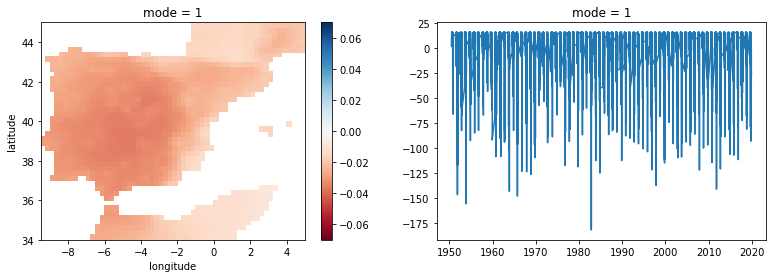
\includegraphics[width=.95\linewidth, height=3cm]{spain-mode1}
    \caption{First PCA mode}
\end{subfigure}%
\begin{subfigure}{.5\textwidth}
    \centering
    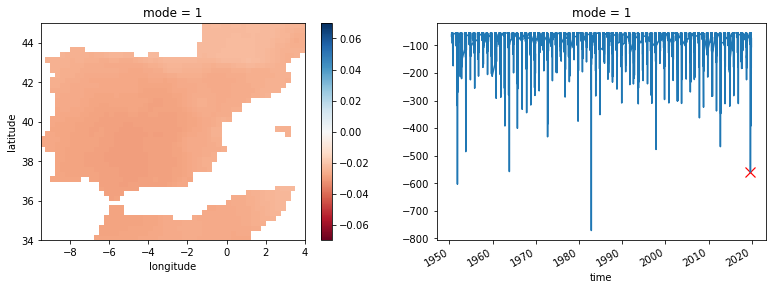
\includegraphics[width=.95\linewidth, height=3cm]{spain-tran-mode1}
    \caption{First xPCA mode}
\end{subfigure}
\end{figure}
\begin{figure}[h!]
\centering
\begin{subfigure}{.5\textwidth}
    \centering
    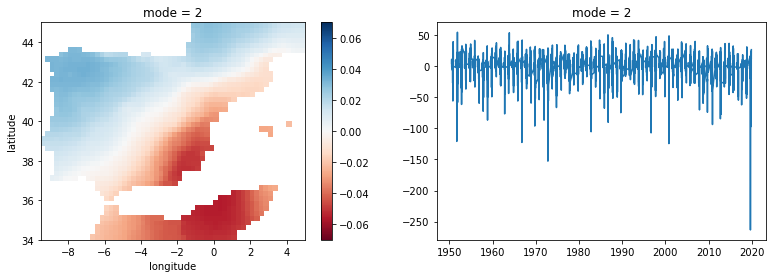
\includegraphics[width=.95\linewidth, height=3cm]{spain-mode2}
    \caption{Second PCA mode}
\end{subfigure}%
\begin{subfigure}{.5\textwidth}
    \centering
    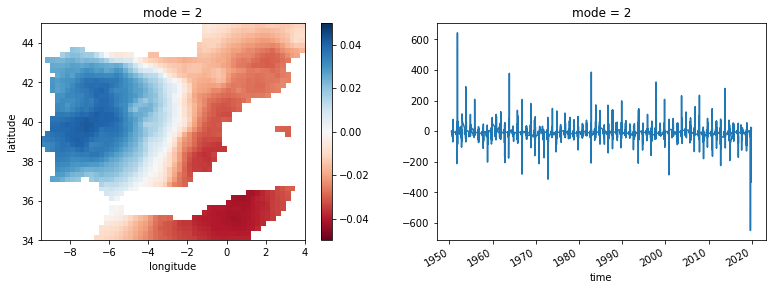
\includegraphics[width=.95\linewidth, height=3cm]{spain-tran-mode2}
    \caption{Second xPCA mode}
\end{subfigure}
\end{figure}
\begin{figure}[h!]
\centering
\begin{subfigure}{.5\textwidth}
    \centering
    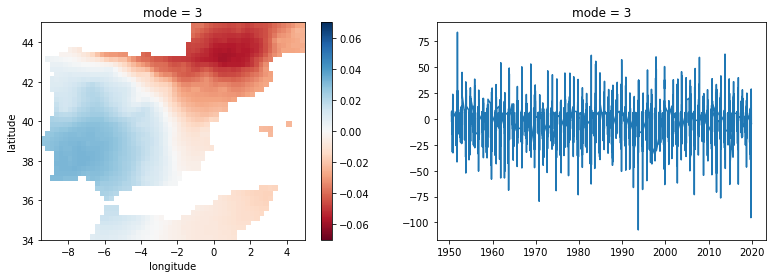
\includegraphics[width=.95\linewidth, height=3cm]{spain-mode3}
    \caption{Third PCA mode}
\end{subfigure}%
\begin{subfigure}{.5\textwidth}
    \centering
    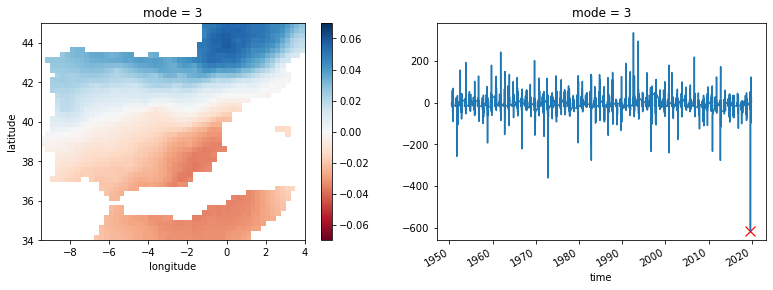
\includegraphics[width=.95\linewidth, height=3cm]{spain-tran-mode3}
    \caption{Third xPCA mode}
\end{subfigure}
\end{figure}
\begin{figure}[h!]
\centering
\begin{subfigure}{.5\textwidth}
    \centering
    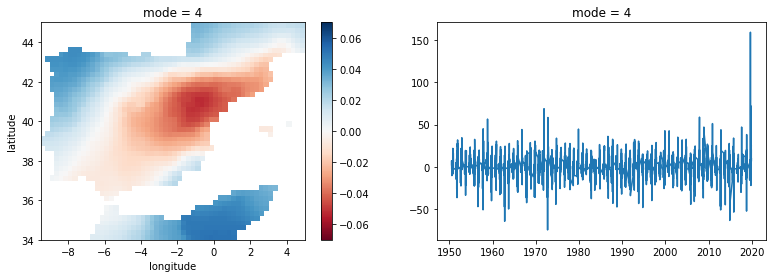
\includegraphics[width=.95\linewidth, height=3cm]{spain-mode4}
    \caption{Fourth PCA mode}
\end{subfigure}%
\begin{subfigure}{.5\textwidth}
    \centering
    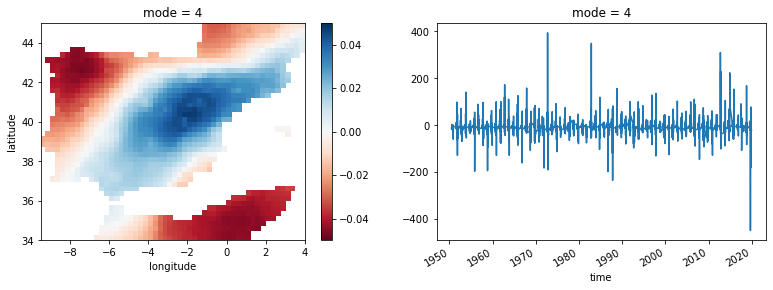
\includegraphics[width=.95\linewidth, height=3cm]{spain-tran-mode4}
    \caption{Fourth xPCA mode}
\end{subfigure}
\end{figure}
\begin{figure}[h!]
\centering
\begin{subfigure}{.5\textwidth}
    \centering
    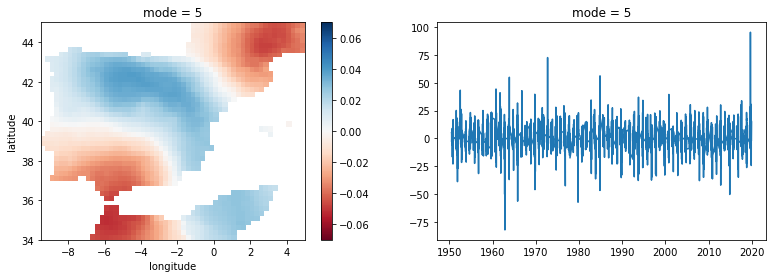
\includegraphics[width=.95\linewidth, height=3cm]{spain-mode5}
    \caption{Fifth PCA mode}
\end{subfigure}%
\begin{subfigure}{.5\textwidth}
    \centering
    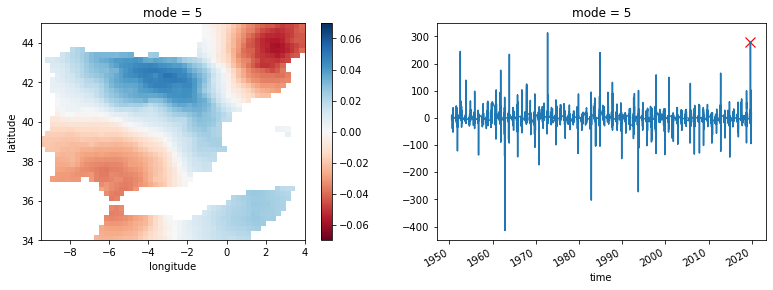
\includegraphics[width=.95\linewidth, height=3cm]{spain-tran-mode5}
    \caption{Fifth xPCA mode}
\end{subfigure}
\end{figure}
\begin{figure}[h!]
\centering
\begin{subfigure}{.5\textwidth}
    \centering
    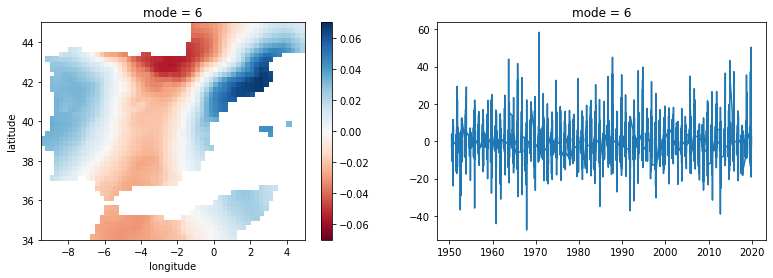
\includegraphics[width=.95\linewidth, height=3cm]{spain-mode6}
    \caption{Sixth PCA mode}
\end{subfigure}%
\begin{subfigure}{.5\textwidth}
    \centering
    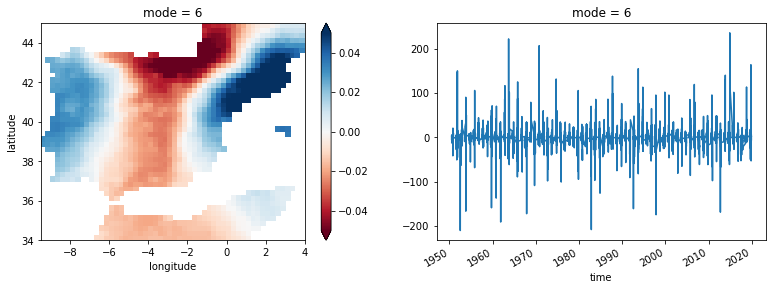
\includegraphics[width=.95\linewidth, height=3cm]{spain-tran-mode6}
    \caption{Sixth xPCA mode}
\end{subfigure}
\end{figure}
\begin{figure}[h!]
\centering
\begin{subfigure}{.5\textwidth}
    \centering
    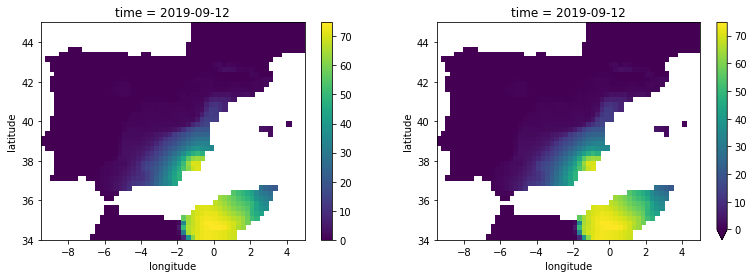
\includegraphics[width=.95\linewidth, height=3cm]{spain-rec}
    \caption{Reconstruction of precipitation using xPCA}
\end{subfigure}%
\begin{subfigure}{.5\textwidth}
    \centering
    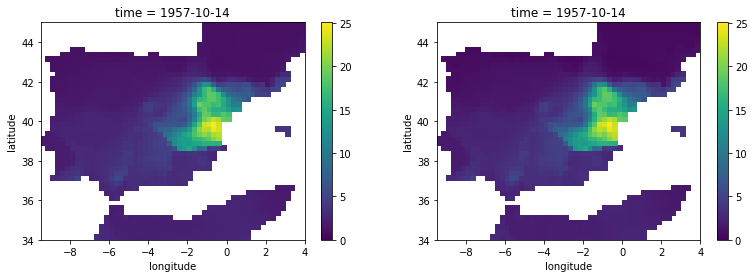
\includegraphics[width=.95\linewidth, height=3cm]{spain-tran-rec}
    \caption{Reconstruction of precipitation using xPCA}
\end{subfigure}
\end{figure}

\subsection{Valencian Country}
Now that we have investigated the behaviour of the PCs in the whole Iberian
Peninsula both for the standard and the extreme PCA methods, we will make a zoom
and focus on a small region, the Valencian Country. Recall that we decided to
investigate extreme events during the Cold Drop season of Spain and those
happen mainly in the eastern third of the Iberian Peninsula, so here is the
motivation to choose this region. The interpretation of the PCs will be very
similar to the one made in the previous case.  

The first eigenvector for both cases again shows a completely negative
homogeneous state along all the region for both cases, which is equivalent to a
complete positive behaviour, due to the complete positiviness of both standard
and extreme covariance matrices. Again, if considered alone the result of this
mode will be that precipitation should be quite homogeneous along all the
region, but when combined with modes that give more weight to some regions
then precipitation will be allocated in these regions.    

Regarding the second and third mode, we see that they're surprisingly very
similar in both cases. The dipole structure that we mentioned in the analysis of
the PCs of the Iberian Peninsula again arises in this case. We see that the
second mode distinguishes between the north and south regions while the third
mode focuses on the interior of the Valencian Country and the mediterranean
coast. Furthemore, something remarkable is that the different of gradient of
values that we appreciated in the Iberian Peninsula now has disappeared and
they're very similar. We note that third mode will therefore have a higher
importance in our case, as it clearly differentiates a homogeneous behaviour on
the east coast.

So as to the fourth, fifth and sixth mode, we see the tripole structure we also
talked about in the previous section. If we pay attention to the fourth and
fifth mode, we can again see that they're similar, except for a sign in the
fifth mode, and that the gradient of values is the same. However, the sixth mode
seems quite different. In the case of the PCA, it does not seem to be very
important as there is no homogeneous behaviour in the east coast, what can be
seen in the sixth xPCA mode. 

We finally include a reconstruction of precipitation events during the day
14/10/1957, where an important flood took place in Valencia. One can note that
the reconstructions are different, but this is again due to the fact that the
preprocessing of the data is different, so the PCA reconstructs the image for
the moving averaged data and the xPCA for the regularly varying transformed
data.

\begin{figure}[h!]
\centering
\begin{subfigure}{.5\textwidth}
    \centering
    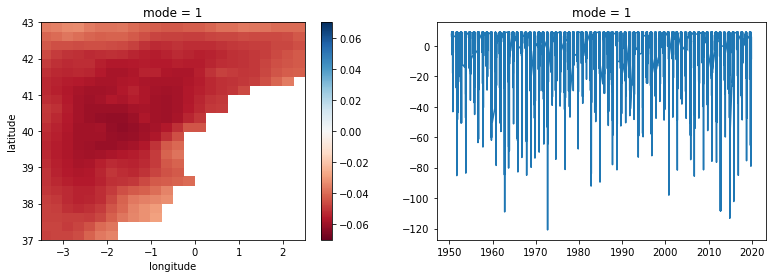
\includegraphics[width=.95\linewidth, height=3cm]{vlc-mode1}
    \caption{First PCA mode}
\end{subfigure}%
\begin{subfigure}{.5\textwidth}
    \centering
    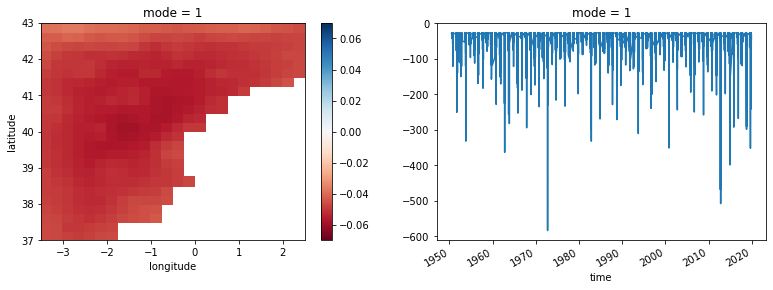
\includegraphics[width=.95\linewidth, height=3cm]{vlc-tran-mode1}
    \caption{First xPCA mode}
\end{subfigure}
\end{figure}
\begin{figure}[h!]
\centering
\begin{subfigure}{.5\textwidth}
    \centering
    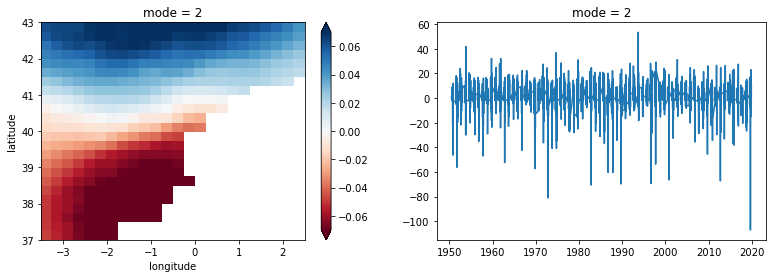
\includegraphics[width=.95\linewidth, height=3cm]{vlc-mode2}
    \caption{Second PCA mode}
\end{subfigure}%
\begin{subfigure}{.5\textwidth}
    \centering
    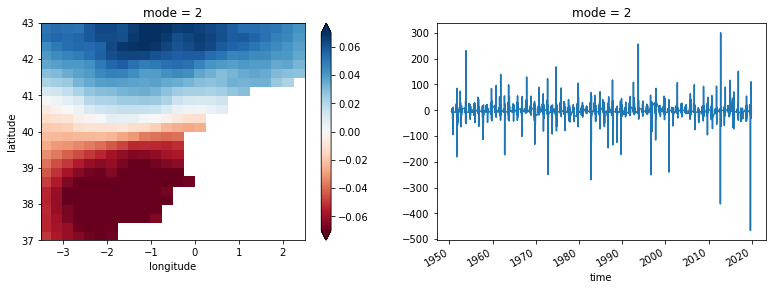
\includegraphics[width=.95\linewidth, height=3cm]{vlc-tran-mode2}
    \caption{Second xPCA mode}
\end{subfigure}
\end{figure}
\begin{figure}[h!]
\centering
\begin{subfigure}{.5\textwidth}
    \centering
    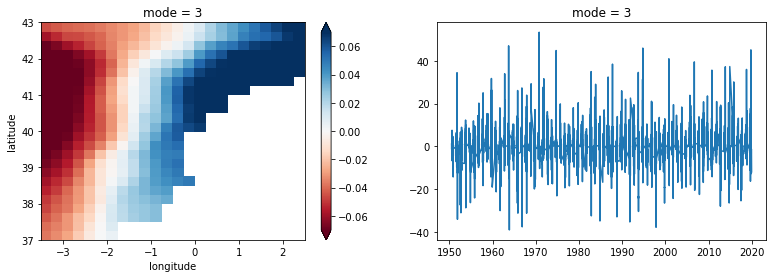
\includegraphics[width=.95\linewidth, height=3cm]{vlc-mode3}
    \caption{Third PCA mode}
\end{subfigure}%
\begin{subfigure}{.5\textwidth}
    \centering
    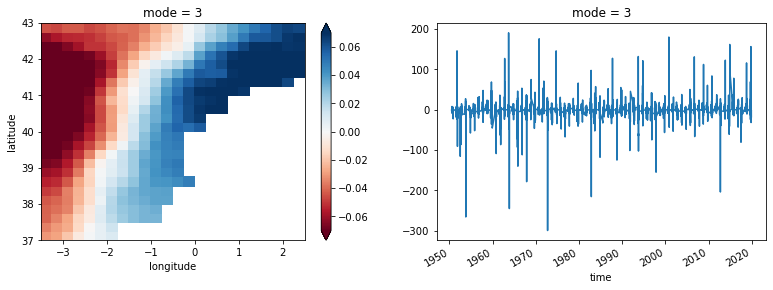
\includegraphics[width=.95\linewidth, height=3cm]{vlc-tran-mode3}
    \caption{Third xPCA mode}
\end{subfigure}
\end{figure}
\begin{figure}[h!]
\centering
\begin{subfigure}{.5\textwidth}
    \centering
    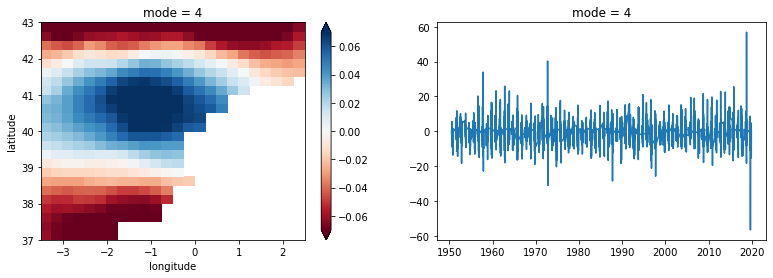
\includegraphics[width=.95\linewidth, height=3cm]{vlc-mode4}
    \caption{Fourth PCA mode}
\end{subfigure}%
\begin{subfigure}{.5\textwidth}
    \centering
    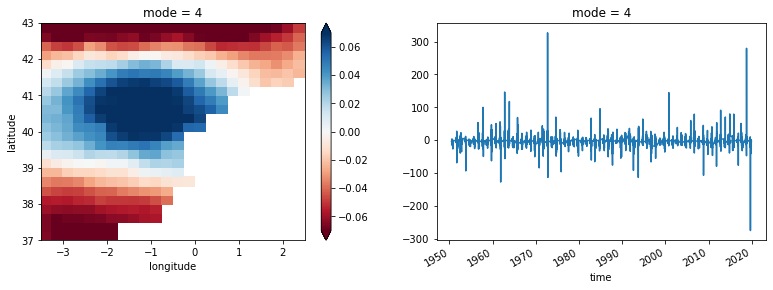
\includegraphics[width=.95\linewidth, height=3cm]{vlc-tran-mode4}
    \caption{Fourth xPCA mode}
\end{subfigure}
\end{figure}
\begin{figure}[h!]
\centering
\begin{subfigure}{.5\textwidth}
    \centering
    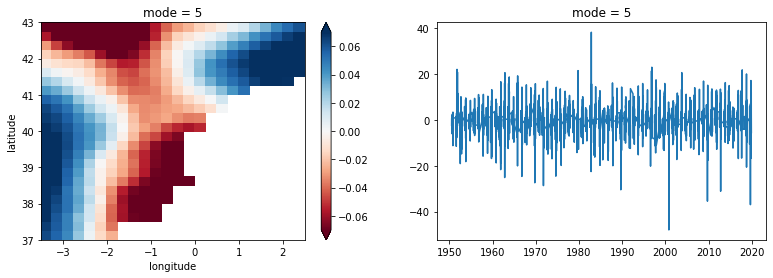
\includegraphics[width=.95\linewidth, height=3cm]{vlc-mode5}
    \caption{Fifth PCA mode}
\end{subfigure}%
\begin{subfigure}{.5\textwidth}
    \centering
    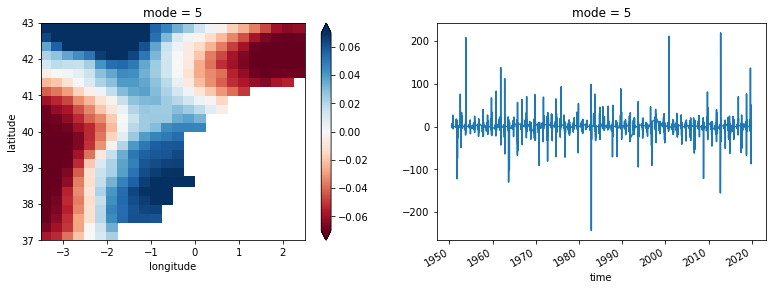
\includegraphics[width=.95\linewidth, height=3cm]{vlc-tran-mode5}
    \caption{Fifth xPCA mode}
\end{subfigure}
\end{figure}
\begin{figure}[h!]
\centering
\begin{subfigure}{.5\textwidth}
    \centering
    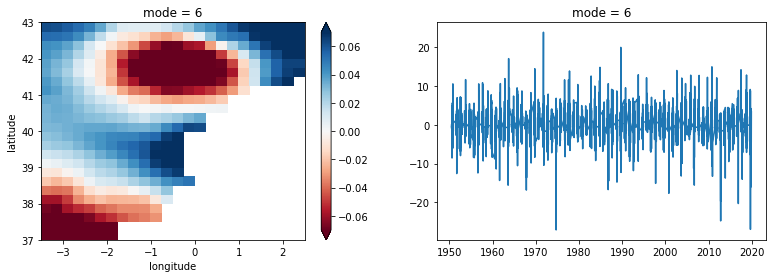
\includegraphics[width=.95\linewidth, height=3cm]{vlc-mode6}
    \caption{Sixth PCA mode}
\end{subfigure}%
\begin{subfigure}{.5\textwidth}
    \centering
    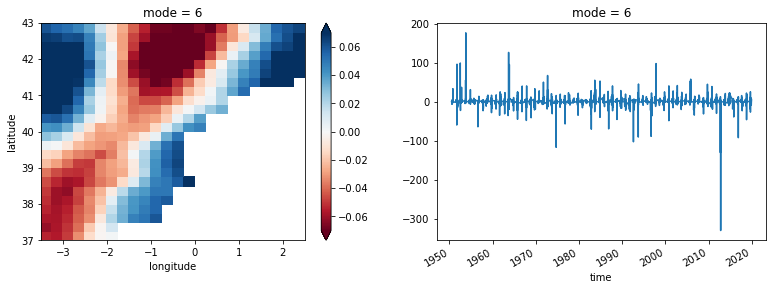
\includegraphics[width=.95\linewidth, height=3cm]{vlc-tran-mode6}
    \caption{Sixth xPCA mode}
\end{subfigure}
\end{figure}
\begin{figure}[h!]
\centering
\begin{subfigure}{.5\textwidth}
    \centering
    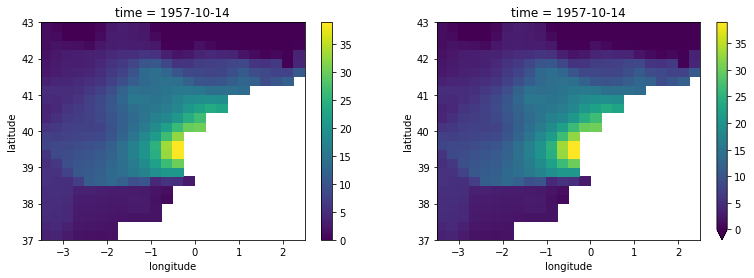
\includegraphics[width=.95\linewidth, height=3cm]{vlc-rec}
    \caption{Reconstruction of precipitation using PCA}
\end{subfigure}%
\begin{subfigure}{.5\textwidth}
    \centering
    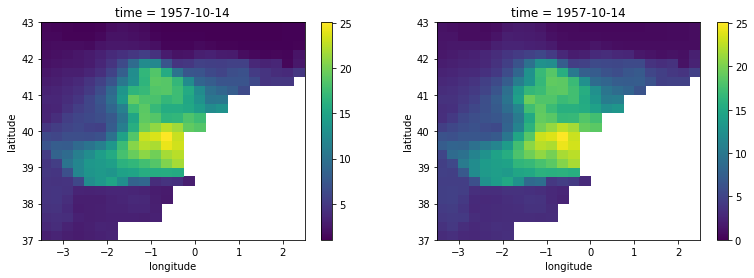
\includegraphics[width=.95\linewidth, height=3cm]{vlc-tran-rec}
    \caption{Reconstruction of precipitation using xPCA}
\end{subfigure}
\end{figure}

\subsection{North America}

\section{Comparison of MCA and xMCA for precipitation and sea surface salinity}
\subsection{Iberian Peninsula and North Atlantic ocean}


\chapter{Discussion}
\chapter{Outlook}


\appendix

%\chapter{About the varied terminology of PCA}\label{chap:terminology-pca}
%Following the discussion in \cite{wilks}, we now discuss the different
%terminology for PCA. The subject of PCA is sometimes regarded as a difficult and
%confusing one, but much of this confusion derives from a proliferation of the
%associated terminology, especially in writings by analysts of atmospheric data.

\chapter{$\mathbb{X}^p$ is a vector space}
Here I will explain that the space that Cooley and Thibaud describe is a vector
space.

\chapter{Code}

\newpage
\printbibliography


  
\end{document}
